\documentclass[12pt]{article}
%DIF LATEXDIFF DIFFERENCE FILE
%DIF DEL /private/tmp/claude-501/-Users-neilpatel/1810e5be-8384-4980-8d1c-8abd20b87fad/scratchpad/manuscript_original_norm.tex   Wed Nov  4 10:50:00 2026
%DIF ADD manuscript_revised.tex                                                                                                  Wed Nov  4 11:31:20 2026

\usepackage[utf8]{inputenc}
\usepackage[T1]{fontenc}
\usepackage{mathptmx}
\usepackage[margin=1in]{geometry}
\usepackage{setspace}
\usepackage[right]{lineno}
\usepackage{graphicx}
\usepackage{booktabs}
\usepackage{longtable}
\usepackage{array}
\usepackage{caption}
\usepackage[hidelinks]{hyperref}

\captionsetup{font=small, labelfont=bf}
\setlength{\parindent}{0pt}
\setlength{\parskip}{6pt}
\setlength{\emergencystretch}{2em}

\newcolumntype{R}[1]{>{\raggedleft\arraybackslash}p{#1}}
%DIF 22a22
\newcolumntype{L}[1]{>{\raggedright\arraybackslash}p{#1}} %DIF > 
%DIF -------
\newcommand{\deltaauc}{$\Delta$AUC}

\title{}
\date{}
%DIF PREAMBLE EXTENSION ADDED BY LATEXDIFF
%DIF UNDERLINE PREAMBLE %DIF PREAMBLE
\RequirePackage[normalem]{ulem} %DIF PREAMBLE
\RequirePackage{color}\definecolor{RED}{rgb}{1,0,0}\definecolor{BLUE}{rgb}{0,0,1} %DIF PREAMBLE
\providecommand{\DIFaddtex}[1]{{\protect\color{blue}\uwave{#1}}} %DIF PREAMBLE
\providecommand{\DIFdeltex}[1]{{\protect\color{red}\sout{#1}}} %DIF PREAMBLE
%DIF SAFE PREAMBLE %DIF PREAMBLE
\providecommand{\DIFaddbegin}{} %DIF PREAMBLE
\providecommand{\DIFaddend}{} %DIF PREAMBLE
\providecommand{\DIFdelbegin}{} %DIF PREAMBLE
\providecommand{\DIFdelend}{} %DIF PREAMBLE
\providecommand{\DIFmodbegin}{} %DIF PREAMBLE
\providecommand{\DIFmodend}{} %DIF PREAMBLE
%DIF FLOATSAFE PREAMBLE %DIF PREAMBLE
\providecommand{\DIFaddFL}[1]{\DIFadd{#1}} %DIF PREAMBLE
\providecommand{\DIFdelFL}[1]{\DIFdel{#1}} %DIF PREAMBLE
\providecommand{\DIFaddbeginFL}{} %DIF PREAMBLE
\providecommand{\DIFaddendFL}{} %DIF PREAMBLE
\providecommand{\DIFdelbeginFL}{} %DIF PREAMBLE
\providecommand{\DIFdelendFL}{} %DIF PREAMBLE
%DIF HYPERREF PREAMBLE %DIF PREAMBLE
\providecommand{\DIFadd}[1]{\texorpdfstring{\DIFaddtex{#1}}{#1}} %DIF PREAMBLE
\providecommand{\DIFdel}[1]{\texorpdfstring{\DIFdeltex{#1}}{}} %DIF PREAMBLE
\providecommand{\DIFscaledelfig}{0.5}
%DIF HIGHLIGHTGRAPHICS PREAMBLE %DIF PREAMBLE
\RequirePackage{settobox} %DIF PREAMBLE
\RequirePackage{letltxmacro} %DIF PREAMBLE
\newsavebox{\DIFdelgraphicsbox} %DIF PREAMBLE
\newlength{\DIFdelgraphicswidth} %DIF PREAMBLE
\newlength{\DIFdelgraphicsheight} %DIF PREAMBLE
% store original definition of \includegraphics %DIF PREAMBLE
\LetLtxMacro{\DIFOincludegraphics}{\includegraphics} %DIF PREAMBLE
\providecommand{\DIFaddincludegraphics}[2][]{{\color{blue}\fbox{\DIFOincludegraphics[#1]{#2}}}} %DIF PREAMBLE
\providecommand{\DIFdelincludegraphics}[2][]{% %DIF PREAMBLE
\sbox{\DIFdelgraphicsbox}{\DIFOincludegraphics[#1]{#2}}% %DIF PREAMBLE
\settoboxwidth{\DIFdelgraphicswidth}{\DIFdelgraphicsbox} %DIF PREAMBLE
\settoboxtotalheight{\DIFdelgraphicsheight}{\DIFdelgraphicsbox} %DIF PREAMBLE
\scalebox{\DIFscaledelfig}{% %DIF PREAMBLE
\parbox[b]{\DIFdelgraphicswidth}{\usebox{\DIFdelgraphicsbox}\\[-\baselineskip] \rule{\DIFdelgraphicswidth}{0em}}\llap{\resizebox{\DIFdelgraphicswidth}{\DIFdelgraphicsheight}{% %DIF PREAMBLE
\setlength{\unitlength}{\DIFdelgraphicswidth}% %DIF PREAMBLE
\begin{picture}(1,1)% %DIF PREAMBLE
\thicklines\linethickness{2pt} %DIF PREAMBLE
{\color[rgb]{1,0,0}\put(0,0){\framebox(1,1){}}}% %DIF PREAMBLE
{\color[rgb]{1,0,0}\put(0,0){\line( 1,1){1}}}% %DIF PREAMBLE
{\color[rgb]{1,0,0}\put(0,1){\line(1,-1){1}}}% %DIF PREAMBLE
\end{picture}% %DIF PREAMBLE
}\hspace*{3pt}}} %DIF PREAMBLE
} %DIF PREAMBLE
\LetLtxMacro{\DIFOaddbegin}{\DIFaddbegin} %DIF PREAMBLE
\LetLtxMacro{\DIFOaddend}{\DIFaddend} %DIF PREAMBLE
\LetLtxMacro{\DIFOdelbegin}{\DIFdelbegin} %DIF PREAMBLE
\LetLtxMacro{\DIFOdelend}{\DIFdelend} %DIF PREAMBLE
\DeclareRobustCommand{\DIFaddbegin}{\DIFOaddbegin \let\includegraphics\DIFaddincludegraphics} %DIF PREAMBLE
\DeclareRobustCommand{\DIFaddend}{\DIFOaddend \let\includegraphics\DIFOincludegraphics} %DIF PREAMBLE
\DeclareRobustCommand{\DIFdelbegin}{\DIFOdelbegin \let\includegraphics\DIFdelincludegraphics} %DIF PREAMBLE
\DeclareRobustCommand{\DIFdelend}{\DIFOaddend \let\includegraphics\DIFOincludegraphics} %DIF PREAMBLE
\LetLtxMacro{\DIFOaddbeginFL}{\DIFaddbeginFL} %DIF PREAMBLE
\LetLtxMacro{\DIFOaddendFL}{\DIFaddendFL} %DIF PREAMBLE
\LetLtxMacro{\DIFOdelbeginFL}{\DIFdelbeginFL} %DIF PREAMBLE
\LetLtxMacro{\DIFOdelendFL}{\DIFdelendFL} %DIF PREAMBLE
\DeclareRobustCommand{\DIFaddbeginFL}{\DIFOaddbeginFL \let\includegraphics\DIFaddincludegraphics} %DIF PREAMBLE
\DeclareRobustCommand{\DIFaddendFL}{\DIFOaddendFL \let\includegraphics\DIFOincludegraphics} %DIF PREAMBLE
\DeclareRobustCommand{\DIFdelbeginFL}{\DIFOdelbeginFL \let\includegraphics\DIFdelincludegraphics} %DIF PREAMBLE
\DeclareRobustCommand{\DIFdelendFL}{\DIFOaddendFL \let\includegraphics\DIFOincludegraphics} %DIF PREAMBLE
%DIF END PREAMBLE EXTENSION ADDED BY LATEXDIFF

\begin{document}
\linenumbers

% ============================================================
% TITLE PAGE
% ============================================================
\begin{singlespace}
\begin{center}
{\Large\bfseries \DIFdelbegin \DIFdel{Reported biomarker-cognition associations do not translate into predictive utility}\DIFdelend \DIFaddbegin \DIFadd{Blood metal and nutritional biomarkers did not improve identification of low cognitive performance beyond demographics in older US adults}\DIFaddend : a pre-registered analysis of NHANES 2011-2014\par}
\end{center}

\bigskip

\begin{center}
Shreyan Kancharla$^{1,\ast}$, Neil Patel$^{2,\ast}$
\end{center}

\medskip

\noindent $^{\ast}$These authors contributed equally to this work and share first authorship.

\medskip

\noindent $^{1}$Davidson College, Davidson, NC, USA.

\noindent $^{2}$University of North Carolina at Chapel Hill, Chapel Hill, NC, USA.

\medskip

\noindent \textbf{Corresponding author:} Shreyan Kancharla, shkancharla@davidson.edu, ORCID: 0009-0009-8654-110X.

\noindent Neil Patel, ORCID: 0009-0000-6134-5641.

\end{singlespace}

\clearpage

% ============================================================
% ABSTRACT
% ============================================================
\doublespacing
\section*{Abstract}

\textbf{Background.} \DIFdelbegin \DIFdel{Multiple studies report associations between blood metals, nutritional biomarkers and cognitive performance among }\DIFdelend \DIFaddbegin \DIFadd{Studies of }\DIFaddend US adults aged 60 and over in the National Health and Nutrition Examination Survey (NHANES) 2011-2014 \DIFaddbegin \DIFadd{report associations between blood metals, nutritional biomarkers and cognitive test performance}\DIFaddend . None isolates the biomarkers' predictive contribution beyond demographics, with calibration and decision-curve analysis.

\textbf{Methods.} We analysed \DIFdelbegin \DIFdel{NHANES 2011-2012 and 2013-2014, restricted to }\DIFdelend examined participants aged 60 and over. Low cognitive performance was \DIFdelbegin \DIFdel{defined as }\DIFdelend the lowest quartile of a composite \DIFdelbegin \DIFdel{z-score }\DIFdelend \DIFaddbegin \DIFadd{of within-sample z-scores }\DIFaddend from CERAD immediate and delayed recall, animal fluency \DIFdelbegin \DIFdel{, }\DIFdelend and the Digit Symbol Substitution Test\DIFdelbegin \DIFdel{. Four nested specifications were pre-specified: }\DIFdelend \DIFaddbegin \DIFadd{: an epidemiologic classification relative to this sample, not a clinical diagnosis. Pre-specified models were }\DIFaddend demographics (M0); demographics plus five blood metals (M1)\DIFdelbegin \DIFdel{; demographics plus }\DIFdelend \DIFaddbegin \DIFadd{, }\DIFaddend fifteen nutritional and metabolic biomarkers (M2)\DIFdelbegin \DIFdel{; and both blocks }\DIFdelend \DIFaddbegin \DIFadd{, or both }\DIFaddend (M3)\DIFdelbegin \DIFdel{. A pre-specified secondary baseline }\DIFdelend \DIFaddbegin \DIFadd{; and demographics plus eight clinical covariates }\DIFaddend (M0+)\DIFdelbegin \DIFdel{added eight routinely recorded clinical covariates}\DIFdelend \DIFaddbegin \DIFadd{. At peer review we added M0+ plus both biomarker blocks (M4)}\DIFaddend . Three algorithms \DIFdelbegin \DIFdel{(L2-penalized logistic regression, random forest, gradient boosting) }\DIFdelend were evaluated by 5$\times$10-fold \DIFdelbegin \DIFdel{stratified }\DIFdelend cross-validation, with preprocessing and tuning \DIFdelbegin \DIFdel{fitted }\DIFdelend inside training folds. The pre-specified primary \DIFdelbegin \DIFdel{measure was \deltaauc(}\DIFdelend \DIFaddbegin \DIFadd{test was superiority of }\DIFaddend M3 \DIFdelbegin \DIFdel{$-$ }\DIFdelend \DIFaddbegin \DIFadd{over }\DIFaddend M0 \DIFdelbegin \DIFdel{) with a 2,000-sample }\DIFdelend \DIFaddbegin \DIFadd{in AUC, with a }\DIFaddend paired bootstrap interval\DIFdelbegin \DIFdel{; 0.02 was pre-specified as the smallest meaningful improvement.
Reporting follows TRIPOD+AI.
}\DIFdelend \DIFaddbegin \DIFadd{.
}\DIFaddend 

\textbf{Results.} Of 3,124 participants with an outcome label, 1,784 had complete predictor data, of whom 431 (24.2\%) \DIFdelbegin \DIFdel{met the definition of }\DIFdelend \DIFaddbegin \DIFadd{had }\DIFaddend low cognitive performance. Demographics alone reached an AUC of 0.788. \deltaauc(M3 $-$ M0) was $-0.0019$ (95\% CI $-0.0108$ to $0.0071$), \DIFdelbegin \DIFdel{with the upper bound below the pre-specified 0.02 threshold; neither biomarker block contributed alone. M3 performed worse than the clinical baseline }\DIFdelend \DIFaddbegin \DIFadd{so superiority was not supported, and adding the biomarkers to }\DIFaddend M0+ \DIFaddbegin \DIFadd{did not improve discrimination either }\DIFaddend (\deltaauc\ \DIFdelbegin \DIFdel{$-0.0158$, 95\% CI $-0.0295$ to $-0.0033$)across all three algorithms, and decision-curve analysis showed no net benefit at any threshold. Quantile g-computation on the metal mixture matched demographics alone (AUC 0.7874). The null persisted across all six }\DIFdelend \DIFaddbegin \DIFadd{$-0.0037$, $-0.0112$ to $0.0029$). In post hoc margin analyses the primary analysis excluded improvements above $0.0056$, but the 10th-percentile analysis excluded only improvements above $0.0132$. Clinical covariates added $0.0139$ ($0.0026$ to $0.0255$) to demographics (post hoc). \deltaauc(M3 $-$ M0) was similar in every }\DIFaddend pre-specified sensitivity \DIFdelbegin \DIFdel{analyses, including multiple imputation on the full sample ($n=3{,}124$; \deltaauc\ 0.0015, 95\% CI $-0.0030$ to $0.0063$) }\DIFdelend \DIFaddbegin \DIFadd{analysis that re-estimated it and among participants with all four cognitive scores. With a post hoc demographically adjusted outcome, all models discriminated poorly; the biomarkers improved on demographics ($0.0362$, $0.0068$ to $0.0667$) but not on M0+}\DIFaddend .

\textbf{Conclusions.} \DIFdelbegin \DIFdel{Reported biomarker-cognition associations did not translate into individual-level predictive utility beyond age, education and income, and a twenty-analyte laboratory panel was outperformed by eight items of routine clinical history. Because the confidence interval excludes the improvement }\DIFdelend \DIFaddbegin \DIFadd{For the }\DIFaddend pre-specified \DIFdelbegin \DIFdel{as meaningful, this is a precise null rather than an inconclusive one}\DIFdelend \DIFaddbegin \DIFadd{outcome, adding twenty blood biomarkers to demographics, or to demographics plus clinical history, did not improve identification of low cognitive performance. The study tested superiority and was not designed to exclude small improvements. Whether they inform performance lower than demographically expected needs confirmation}\DIFaddend .

\medskip
\noindent\textbf{Keywords:} Cognitive performance; biomarkers; blood metals; prediction model; NHANES; older adults; TRIPOD+AI; decision-curve analysis; pre-registration; machine learning

\clearpage

% ============================================================
% BACKGROUND
% ============================================================
\section*{Background}

Low cognitive performance in older adults is examined routinely against blood metals and nutritional biomarkers in the National Health and Nutrition Examination Survey (NHANES), and panels of these analytes are proposed periodically as adjuncts to demographic risk assessment. Every \DIFdelbegin \DIFdel{study making that case }\DIFdelend \DIFaddbegin \DIFadd{association study we identified }\DIFaddend for the population and cycles examined here, however, reports only a regression coefficient or an odds ratio. None reports whether the association translates into the ability to identify, at the level of one participant, who has low cognitive performance, and none benchmarks that ability against what is already known from a person's age, sex, race and Hispanic origin, education and family income.

Seven studies span the NHANES 2011-2014 cycles and the population aged 60 years or older analysed here, and none closes that gap. In a preprint, Wang et al.\ examined blood lead, cadmium, mercury, selenium and manganese in 1,460 participants using linear regression and restricted cubic splines [1]. Lu et al.\ added serum iron to the same five metals in 2,002 participants using weighted logistic regression [2]. Tang et al.\ evaluated the same five metals against a dietary inflammatory index in 1,726 participants, using a generalised linear model alongside three mixture-modelling methods: Bayesian kernel machine regression, weighted quantile sum regression and quantile g-computation [3]. Fu et al.\ examined lead, cadmium, mercury, selenium, copper and zinc jointly in 811 participants using quantile regression and Bayesian kernel machine regression [4]. Song et al.\ examined the same class of mixture in 1,833 participants stratified by sex [5]. Laouali et al.\ applied quantile g-computation to lead, cadmium and manganese in 1,777 participants, testing effect modification by two measures of diet quality [6]. Huang and Ren examined an interaction between blood cadmium and dietary omega-6 fatty acid intake in 1,918 participants using logistic regression [7]. \DIFdelbegin \DIFdel{Not one }\DIFdelend \DIFaddbegin \DIFadd{None }\DIFaddend of the seven reports discrimination, calibration or cross-validation, and \DIFdelbegin \DIFdel{not one }\DIFdelend \DIFaddbegin \DIFadd{none }\DIFaddend compares a biomarker-containing model against a demographics-only baseline.

\DIFdelbegin \DIFdel{This is a different question , not a different exposure. Adding one more metal or biomarker to an already saturated association literature is incremental; asking whether any of it predicts, at the individual level and benchmarked against demographics }\DIFdelend \DIFaddbegin \DIFadd{The question addressed here therefore differs from that of the association studies: not whether a biomarker is associated with cognitive test performance, but whether measuring it improves the identification of individuals with low performance beyond what demographics already provide. A strong association does not imply useful discrimination, because the area under the receiver operating characteristic curve (AUC) changes little when even strongly associated markers are added to a model }[\DIFadd{10}\DIFaddend , \DIFdelbegin \DIFdel{is categorical}\DIFdelend \DIFaddbegin \DIFadd{11}]\DIFaddend . To our knowledge, \DIFdelbegin \DIFdel{that test }\DIFdelend \DIFaddbegin \DIFadd{this question }\DIFaddend has not previously been \DIFdelbegin \DIFdel{performed on }\DIFdelend \DIFaddbegin \DIFadd{examined in }\DIFaddend this population, with one recent exception\DIFdelbegin \DIFdel{addressed directly here rather than left for the reader to find independently}\DIFdelend . Ren et al.\ restricted their sample to NHANES participants aged 60 or older, pooled across the 1999-2000, 2001-2002, 2011-2012 and 2013-2014 cycles, and trained a gradient-boosted model on urinary metals and demographic data to classify what they term ``cognitively impaired'' status, reporting a cross-validated \DIFdelbegin \DIFdel{area under the receiver operating characteristic curve (AUC ) }\DIFdelend \DIFaddbegin \DIFadd{AUC }\DIFaddend of 0.90 [8]. Two things distinguish the present study from theirs. First, NHANES contains no clinical diagnosis of cognitive impairment; the outcome available is a \DIFdelbegin \DIFdel{low-performance classification against normed test scores}\DIFdelend \DIFaddbegin \DIFadd{classification of low test performance relative to the distribution of scores within the survey sample}\DIFaddend , which we term \textbf{low cognitive performance} throughout, and we do not adopt their terminology. Second, \DIFdelbegin \DIFdel{and more consequentially for the question this study asks, }\DIFdelend Ren et al.\ report the discrimination of one combined model\DIFdelbegin \DIFdel{and stop there}\DIFdelend : their analysis does not decompose that AUC into what demographics alone would achieve and what the metals add beyond it. That decomposition \DIFdelbegin \DIFdel{, not combined-model discrimination in isolation, }\DIFdelend is the quantity a demographics-only baseline is built to measure, and it is what this study reports. A second study, by Nabavi et al., trained a stacking ensemble on heavy-metal biomarkers to predict \DIFdelbegin \DIFdel{cognitive impairment }\DIFdelend \DIFaddbegin \DIFadd{what they term ``cognitive impairment'' }\DIFaddend across all adults aged 20 and older, reporting an AUC of 0.778, but its population falls outside the age range examined here and it does not report a demographics-only baseline either [9].

The gap between statistical association and predictive utility is a recognised methodological problem beyond this specific exposure-outcome pair, and reporting standards have moved to reflect it: the TRIPOD+AI statement now specifies calibration, decision-curve analysis and internal or external validation as expected components of any prediction-model report, for regression or machine-learning methods alike [\DIFdelbegin \DIFdel{10}\DIFdelend \DIFaddbegin \DIFadd{12}\DIFaddend ]. None of the association studies above provide any of these. This study does, reported against the TRIPOD+AI checklist in full.

Two limits to this novelty claim are stated here rather than left implicit. The data are not novel: NHANES 2011-2014 is a heavily analysed dataset. The algorithms are not novel: penalised logistic regression, random forests and gradient boosting are standard classifiers. The contribution is the question, the evaluation framework built to answer it, and the reporting standard applied to it, not a new exposure, outcome, or method.

\textbf{Objectives.} This study estimates how much predictive value blood metals and nutritional biomarkers add, beyond demographics, for identifying low cognitive performance in US adults aged 60 and older, quantified as the change in cross-validated AUC between a demographics-only model and a model additionally containing the biomarker panel, with calibration and decision-curve analysis reported alongside discrimination. This is a model development study with internal validation by repeated cross-validation; no external validation cohort exists for this exposure-outcome pairing, and this is stated as a limitation below. Hypotheses, the primary metric, the threshold for a meaningful difference, and every sensitivity analysis were fixed in writing before any outcome-predictor relationship was examined, and are reported in full in the pre-registration (Additional file \DIFdelbegin \DIFdel{).
}\DIFdelend \DIFaddbegin \DIFadd{1). Analyses added at peer review are identified as post hoc wherever they are reported, and were recorded in a dated amendment to the pre-registration before they were run.
}\DIFaddend 

% ============================================================
% METHODS
% ============================================================
\section*{Methods}

\subsection*{Study population and design}

We analysed the National Health and Nutrition Examination Survey (NHANES) cycles 2011-2012 and 2013-2014, a complex multistage probability sample of the non-institutionalised civilian US population. Analyses were restricted to participants aged 60 years or older who completed the Mobile Examination Centre visit, the population to whom the cognitive battery was administered. Because two two-year cycles were pooled, the examination weight \texttt{WTMEC2YR} was halved, and the variance strata and primary sampling units were carried through every merge.

The reporting follows TRIPOD+AI. The completed checklist is provided as \DIFdelbegin \DIFdel{a supplementary file .
}\DIFdelend \DIFaddbegin \DIFadd{Additional file 2.
}\DIFaddend 

\subsection*{Outcome}

Cognitive performance was measured with four scores from three instruments: the Consortium to Establish a Registry for Alzheimer's Disease (CERAD) word-list learning task, scored as the sum of three immediate-recall trials and separately as delayed recall; a one-minute animal fluency task; and the Digit Symbol Substitution Test \DIFaddbegin \DIFadd{(DSST) }\DIFaddend from the Wechsler Adult Intelligence Scale III.

Each score was standardised within the pooled sample aged 60 and over. A composite was formed as the mean of the available standardised scores, requiring at least three of four to be present, and the lowest quartile of that composite \DIFaddbegin \DIFadd{(composite $z \le -0.543$) }\DIFaddend defined \textbf{low cognitive performance}. Internal consistency across the four standardised scores was acceptable (Cronbach alpha 0.795); the correlation between CERAD immediate and delayed recall was 0.743, as expected for two scores from one administration, while correlations among the three instruments ranged from 0.40 to 0.51.

\DIFdelbegin \DIFdel{The composite }\DIFdelend \DIFaddbegin \DIFadd{This outcome is an epidemiologic classification, not a clinical one. The scores were standardised within this sample rather than against norms from a cognitively healthy reference group; they were not corrected for age, education or any other demographic characteristic; and the classification takes no account of premorbid ability, change over time, everyday functioning or clinical adjudication. A participant with limited formal schooling can therefore fall in the lowest quartile without any acquired decline, and a participant with high premorbid ability can decline substantially and remain above the cutoff. Because the composite averages whichever three or four scores are available, participants with three scores have composites of different content from those with four. Raw scores, the composite's distribution, language of administration and the number of component scores are reported in Table 1.
}

\DIFadd{The composite }\DIFaddend is defined against pooled-sample quantiles, so a participant's label depends on the distribution of the whole sample. This is a property of the definition rather than of the prediction procedure: the outcome is explicitly relative, and defining it within folds would make the target itself vary between folds. The choice was pre-specified.

\subsection*{Predictors}

Predictors were organised into three blocks fixed in writing before any analysis.

\textbf{Block 1, demographics.} Age, sex, race and Hispanic origin, education, and the family income-to-poverty ratio.

\textbf{Block 2, blood metals.} Lead, cadmium, total mercury, selenium and manganese, measured by inductively coupled plasma mass spectrometry in whole blood, each entered on the natural log scale. Values below the limit of detection are substituted by NHANES with the limit divided by the square root of two and flagged; within the analytic sample this affected 5.2\% of cadmium and 5.7\% of mercury measurements, and no lead, selenium or manganese measurements.

\textbf{Block 3, nutritional and metabolic biomarkers.} Serum vitamin B12, methylmalonic acid, serum total folate, red blood cell folate, 25-hydroxyvitamin D, glycohaemoglobin (HbA1c), high-density lipoprotein (HDL) cholesterol, total cholesterol, triglycerides, albumin, serum iron, estimated glomerular filtration rate (eGFR; CKD-EPI 2021, without the race coefficient), and three inflammation indices derived from the complete blood count: the neutrophil-to-lymphocyte ratio, the platelet-to-lymphocyte ratio, and the systemic immune-inflammation index. Vitamin B12, methylmalonic acid and the systemic immune-inflammation index were log-transformed.

\textbf{Covariates.} \DIFdelbegin \DIFdel{Body mass index, smoking status , }\DIFdelend \DIFaddbegin \DIFadd{Measured body mass index; self-reported smoking status and }\DIFaddend average alcoholic drinks per day\DIFdelbegin \DIFdel{, }\DIFdelend \DIFaddbegin \DIFadd{; }\DIFaddend the nine-item Patient Health Questionnaire depression score\DIFdelbegin \DIFdel{, }\DIFdelend \DIFaddbegin \DIFadd{; }\DIFaddend and self-reported \DIFaddbegin \DIFadd{physician diagnosis of }\DIFaddend stroke, diabetes, hypertension and high cholesterol. These were not entered in the primary nested comparison, which is stated against demographics, but form a pre-specified secondary baseline described below.

\subsection*{Data preparation}

Reserved codes for refusal and non-response were converted to missing on a per-variable basis against each variable's own codebook rather than by a blanket rule, because the applicable codes differ: alcohol quantity uses 777 and 999 over a valid range of 1 to 82, while the cognitive score variables carry no reserved codes at all and a blanket rule would have deleted valid scores of 7 and 9.

Two data properties required specific handling and are noted because both fail silently. First, NHANES SAS transport files encode zero as a denormalised floating-point value rather than as zero, in 330,496 cells across the files used here, with no true zero present anywhere; any equality test against zero therefore matches nothing until this is normalised. Second, alcohol consumption is governed by two nested skip patterns: the screening question refers to any one year of life rather than the past year, and the quantity item is skipped whenever the frequency item is zero. Both indicate zero consumption rather than unknown consumption, and 403 participants were affected.

Derived quantities used in modelling (log transforms, ratios, estimated glomerular filtration rate, depression score) are row-wise functions with no fitted parameters and were computed before splitting; all fitted transformations are described below.

\subsection*{Models}

Four nested models were specified in advance:

\begin{itemize}
\item \textbf{M0}, demographics alone, the benchmark against which everything is measured
\item \textbf{M1}, demographics plus blood metals
\item \textbf{M2}, demographics plus nutritional and metabolic biomarkers
\item \textbf{M3}, demographics plus both biomarker blocks
\end{itemize}

A fifth, pre-specified secondary model\DIFaddbegin \DIFadd{, }\DIFaddend \textbf{M0+}\DIFaddbegin \DIFadd{, }\DIFaddend comprised demographics plus the \DIFaddbegin \DIFadd{eight }\DIFaddend covariates listed above\DIFdelbegin \DIFdel{, representing information a clinician could record without a laboratory. }\DIFdelend \DIFaddbegin \DIFadd{: a demographic-plus-clinical-history baseline. M0+ is not laboratory-free. Diabetes, hypertension and high cholesterol are in routine practice established by laboratory testing or clinical measurement, and overlap in content with HbA1c and the lipid measures in M3, and body mass index is a measured anthropometric rather than an item of history. M3 and M0+ are also not nested: each adds a different set of variables to demographics, so their comparison contrasts two sources of information and cannot show whether the biomarkers add anything to clinical history. To answer that question on nested models, a sixth model, }\textbf{\DIFadd{M4}}\DIFadd{, comprising M0+ plus both biomarker blocks (33 features), was added at peer review (post hoc).
}\DIFaddend 

The cross-validated performance estimates below come from the nested-CV procedure \DIFdelbegin \DIFdel{just described }\DIFdelend \DIFaddbegin \DIFadd{described under Evaluation}\DIFaddend , in which each of the 50 folds fits its own pipeline; no single coefficient set exists from that procedure. For reporting compliance, the identical M3 pipeline was separately refit on the complete analytic sample, with the regularisation strength selected by the same grid via 10-fold cross-validation on the full sample (which selected $C=0.1$, matching the mode across the original 50 folds). Standardised coefficients, odds ratios, and 2,000-resample bootstrap 95\% CIs from that refit are reported in full in \DIFdelbegin \DIFdel{a supplementary table.
}\DIFdelend \DIFaddbegin \DIFadd{Additional file 3.
}\DIFaddend 

Three algorithms were fitted to each specification: L2-penalized logistic regression as the pre-specified primary model class, random forest, and gradient boosting (XGBoost). Multilayer perceptron and k-nearest-neighbour models were excluded in advance, as they were not expected to be competitive at this sample size.

\subsection*{Analytic sample}

All models were fitted and evaluated on a single locked set of rows, those with every Block 1 to 3 predictor and every covariate observed. Fitting nested models on different samples would confound model content with sample composition and render the primary contrast uninterpretable. Nothing was imputed in the primary analysis, so the exposures of interest were never fabricated.

\subsection*{Evaluation}

Models were evaluated by stratified 10-fold cross-validation repeated five times. Every preprocessing step (imputation, standardisation, one-hot encoding) and all hyperparameter selection were performed inside the training folds using pipeline objects constructed within the cross-validation loop; no transformation was fitted on data used for evaluation. This was verified by an automated audit that refits a fold and asserts that the fitted standardisation parameters equal the training-fold values and not the full-sample values; the audit fails the analysis rather than issuing a warning, and it passed.

Discrimination was summarised by the \DIFdelbegin \DIFdel{area under the receiver operating characteristic curve (AUC ) }\DIFdelend \DIFaddbegin \DIFadd{AUC }\DIFaddend and the area under the precision-recall curve, overall accuracy being uninformative at this prevalence. Calibration was summarised by the calibration slope and the calibration-in-the-large intercept, the latter obtained from the offset model rather than by the common shortcut of subtracting the mean linear predictor from an intercept-only fit. Clinical utility was assessed by decision-curve analysis across threshold probabilities from 0.05 to 0.60.

The pre-specified primary outcome measure was \textbf{\deltaauc\ between M3 and M0}, with a 95\% confidence interval from 2,000 bootstrap resamples of participants, scoring both models on the same resampled rows so that the comparison remains paired. \DIFaddbegin \DIFadd{The pre-registered primary hypothesis was a superiority test: that this interval would exclude zero. }\DIFaddend A difference of \DIFdelbegin \DIFdel{at least }\DIFdelend 0.02 in AUC was \DIFaddbegin \DIFadd{also }\DIFaddend declared in advance \DIFaddbegin \DIFadd{as the smallest improvement to be regarded as meaningful, but no equivalence or non-superiority test was pre-specified, and the value 0.02 was the investigators' judgement rather than a value derived from a clinical decision, from comparison with established models or from published evidence on meaningful AUC differences. We are not aware of an accepted minimal important difference in AUC for this purpose. The study was therefore designed to test superiority, not to exclude a meaningful effect, and 0.02 is treated below as one of several candidate margins rather than as a decision rule.
}

\subsection*{\DIFadd{Analyses added at peer review}}

\DIFadd{The analyses in this subsection are post hoc. They were requested at peer review, were recorded in a dated amendment to the pre-registration before they were run (Additional file 1), and are reported as exploratory.
}

\textbf{\DIFadd{Margin analysis.}} \DIFadd{For \deltaauc(M3 $-$ M0) in the primary analysis and in each sensitivity analysis, we report the 90\% paired-bootstrap interval, taken from the same 2,000 resamples as the 95\% interval. At candidate margins $\delta$ of 0.01, 0.015 and 0.02, an improvement of $\delta$ or more is excluded at the one-sided 5\% level when the upper 90\% bound lies below $\delta$, and equivalence within $\pm\delta$ is shown by two one-sided tests when the whole 90\% interval lies within $(-\delta, \delta)$ }[\DIFadd{13, 14}]\DIFadd{. We also report the smallest improvement each analysis excludes, which is its upper 90\% bound, so that readers can apply a margin of their own.
}

\textbf{\DIFadd{All pairwise contrasts.}} \DIFadd{\deltaauc\ with 95\% and 90\% intervals for every pair of the six models under each algorithm, including the clinical covariates added to demographics (M0+ $-$ M0), which was not pre-specified, and for each nonlinear learner against logistic regression within each model. The 0.02 criterion is applied symmetrically: a difference in either direction is not described as meaningful unless its 95\% interval lies wholly beyond 0.02 in magnitude.
}

\textbf{\DIFadd{M4}}\DIFadd{, as defined above, fitted with the same three algorithms, nested cross-validation, seed and locked rows as M0 }\DIFaddend to \DIFdelbegin \DIFdel{be the smallest meaningful improvement}\DIFdelend \DIFaddbegin \DIFadd{M0+}\DIFaddend .

\DIFaddbegin \textbf{\DIFadd{Complete cognitive battery.}} \DIFadd{Restriction to participants with all four component scores, retaining the primary label.
}

\textbf{\DIFadd{Demographically adjusted outcome.}} \DIFadd{Regression-based norms derived within the sample. The composite was regressed by ordinary least squares on age, age squared, sex, education and race and Hispanic origin among the 3,120 labelled participants with complete demographic data, and the lowest quartile of the residual defined performance lower than expected for demographic background. Income was not included, as it is not a conventional norming variable, so M0, which contains income, retains some discrimination on this outcome. Like the primary label, this label was defined on the pooled labelled sample rather than within folds. Externally derived norms were not applied: the published norms for these instruments come from different reference populations and administration formats, and none covers all four scores as administered in NHANES in English, Spanish and Asian languages.
}

\textbf{\DIFadd{Outcome construction.}} \DIFadd{Missing cognitive scores by test, by the NHANES reason code and by demographic group; participants with three against four component scores; and labelled against unlabelled participants.
}

\textbf{\DIFadd{Continuous outcome.}} \DIFadd{A paired bootstrap 95\% interval for the change in cross-validated R-squared.
}

\DIFadd{The complete-battery and demographically adjusted analyses used the primary tuned logistic regression pipeline.
}

\DIFaddend \subsection*{Mixture-modelling benchmark}

To compare the methods used in environmental epidemiology against machine learning on predictive rather than inferential criteria, quantile g-computation was reimplemented in Python. Exposures are quantised into quartiles using cutpoints learned on the training fold and applied unchanged to held-out data, matching the behaviour of the R implementation and preserving fold isolation. The joint mixture effect is the sum of the exposure coefficients, and component weights are the signed coefficients normalised within direction.

Bayesian kernel machine regression was excluded in advance\DIFdelbegin \DIFdel{: a 2026 simulation study of its probit implementation reported that only 30 of 431 fits met standard convergence criteria for binary outcomes, and }\DIFdelend \DIFaddbegin \DIFadd{, because }\DIFaddend refitting a Markov chain Monte Carlo model inside \DIFaddbegin \DIFadd{each of the }\DIFaddend 50 \DIFaddbegin \DIFadd{cross-validation }\DIFaddend folds was not feasible within the analysis budget. Weighted quantile sum regression was deferred, its package partitioning data internally in a way that conflicts with an external cross-validation scheme.

\subsection*{Interpretation}

SHAP values were computed for the gradient-boosted M3 model, with feature rankings recomputed across 200 bootstrap resamples to characterise rank stability, since single-run rankings over correlated predictors are not reliable. Partial dependence was examined for selenium and manganese, the two exposures for which non-monotonic exposure-response was anticipated.

\subsection*{Sensitivity analyses}

Six analyses were specified in advance: outcome cutoffs at the 10th and 20th percentiles; the continuous composite as a regression outcome; recoding participants unable to complete the Digit Symbol Substitution Test as having low performance; restriction to English-language administration; multiple imputation by chained equations on the full labelled sample with imputation fitted inside folds; and a leave-one-block-out comparison. \DIFaddbegin \DIFadd{These used L2-penalized logistic regression with a fixed penalty ($C = 1$) rather than inner-loop tuning; on the primary specification this pipeline gives \deltaauc(M3 $-$ M0) $= -0.0020$ (95\% CI $-0.0103$ to $0.0066$), differing from the primary estimate by about 0.0001.
}\DIFaddend 

\subsection*{Software and reproducibility}

Analyses used Python 3.12.2 with pandas 3.0.3, scikit-learn 1.8.0, XGBoost 3.0.0, SciPy 1.13.0 and SHAP 0.52.0. All random seeds were fixed at a single master value and package versions are pinned. The complete pipeline, from file acquisition through figures, is available as \DIFdelbegin \DIFdel{seven independently runnable scripts}\DIFdelend \DIFaddbegin \DIFadd{independently runnable numbered scripts, including those for the analyses added at peer review}\DIFaddend .

% ============================================================
% RESULTS
% ============================================================
\section*{Results}

\subsection*{Participants}

Of 19,931 participants in the two cycles, 3,632 were aged 60 or older and 3,472 had completed the examination visit. Of these, 3,124 had at least three of four cognitive scores and received an outcome label. Requiring complete data on all predictors and covariates yielded the analytic sample of \textbf{1,784 participants, of whom 431 (24.2\%) met the definition of low cognitive performance}. The \DIFdelbegin \DIFdel{weighted population represented was }\DIFdelend \DIFaddbegin \DIFadd{3,472 examined participants represented a weighted population of }\DIFaddend 59.7 million. Participant flow through each stage is shown in Fig.~\ref{fig:flow}.

The 2013-2014 cycle contributed proportionally fewer participants (661) than 2011-2012 (1,123), because blood metals in that cycle were measured in a one-half random subsample rather than in all examined participants.

Participants excluded for incomplete data were slightly older (mean 70.1 against 69.4 years) and slightly more likely to meet the outcome definition (26.1\% against 24.2\%), with all differences under three percentage points (Table~\ref{tab:t1b}). Participant characteristics for the analytic sample, overall and by outcome status, \DIFaddbegin \DIFadd{including its cognitive phenotype, }\DIFaddend are shown in Table~\ref{tab:t1a}.

\DIFaddbegin \subsection*{\DIFadd{Cognitive data and missingness}}

\DIFadd{Of the 3,472 examined participants, 348 had fewer than three cognitive scores and received no label. Most had no score at all because they were interviewed by proxy (49), were not offered the tests in their language (25) or did no test (202). Unlabelled participants were older (mean (SD) age 72.3 (7.4) against 69.7 (6.8) years), more often had less than high school education (172 (49.4\%) against 846 (27.1\%)) and more often reported a stroke (62 (17.8\%) against 237 (7.6\%)) (Additional file 4, Table S5). The proportion with fewer than three scores was 10.0\% overall but 17.5\% at age 80 and over, 22.1\% among non-Hispanic Asian participants and 22.5\% among those with less than 9th-grade education (Table S3).
}

\DIFadd{The DSST was the score most often missing (458 of 3,472; Table S2). Beyond participants who were not tested at all, its reason codes were communication problem (11), physical limitation (22), refusal (34) and other (2), and 113 missing DSST scores had no reason recorded. These codes cannot separate sensory, motor, comprehension or administration barriers from cognitive limitation.
}

\DIFadd{Within the analytic sample, 90 participants (5.0\%) had three rather than four scores, 64 (71.1\%) of them missing the DSST. Compared with participants with four scores, they were older (mean (SD) age 72.0 (7.1) against 69.2 (6.7) years), more often had less than high school education (47 (52.2\%) against 396 (23.4\%)) and were more often tested in Spanish or an Asian language (22 (24.4\%) against 187 (11.0\%)), and 58 (64.4\%) met the outcome definition against 373 (22.0\%) (Table S4).
}

\DIFaddend \subsection*{Discrimination}

Demographics alone discriminated moderately well (AUC 0.7884). Adding blood metals (M1, 0.7868), nutritional biomarkers (M2, 0.7895), or both (M3, 0.7865) produced no material change. The clinical baseline M0+ reached 0.8023 \DIFaddbegin \DIFadd{and M4 reached 0.7986}\DIFaddend .

\textbf{The primary result was \deltaauc(M3 $-$ M0) $= -0.0019$, with a bootstrap 95\% confidence interval of [$-0.0108$, $0.0071$]} (Fig.~\ref{fig:forest}\DIFaddbegin \DIFadd{, Table~\ref{tab:t3}}\DIFaddend ). The interval includes zero, so the \DIFdelbegin \DIFdel{primary }\DIFdelend \DIFaddbegin \DIFadd{pre-specified superiority }\DIFaddend hypothesis was not supported. \DIFdelbegin \DIFdel{Its upper bound of 0.0071 falls below the 0.02 threshold declared in advance, so the analysis excludes an improvement of the magnitude specified as meaningful rather than merely failing to detect one.
}%DIFDELCMD < 

%DIFDELCMD < %%%
\DIFdelend Neither block contributed individually: \deltaauc\ was $-0.0015$ [$-0.0052$, $0.0023$] for metals and $0.0011$ [$-0.0067$, $0.0100$] for nutritional biomarkers.
\DIFdelbegin \DIFdel{The question of non-redundancy between blocks does not arise. }\DIFdelend 

\DIFdelbegin \DIFdel{The one contrast whose interval excluded zero was negative. }\textbf{\DIFdel{M3 performed worse than the clinical baseline M0+}}%DIFAUXCMD
\DIFdel{, by $-0.0158$ }\DIFdelend \DIFaddbegin \DIFadd{On nested models, adding both biomarker blocks to the clinical baseline did not improve discrimination either (post hoc). \deltaauc(M4 $-$ M0+) was $-0.0037$ }\DIFaddend [\DIFdelbegin \DIFdel{$-0.0295$, $-0.0033$}\DIFdelend \DIFaddbegin \DIFadd{$-0.0112$, $0.0029$}\DIFaddend ] \DIFaddbegin \DIFadd{under logistic regression, $-0.0093$ }[\DIFadd{$-0.0196$, $0.0013$}] \DIFadd{under random forest and $-0.0093$ }[\DIFadd{$-0.0201$, $0.0018$}] \DIFadd{under gradient boosting. Under the two nonlinear learners M4 was, if anything, slightly worse than M0+: their 90\% intervals lay just below zero (Table S6).
}

\DIFadd{Adding the eight clinical covariates to demographics (post hoc) increased AUC by $0.0139$ }[\DIFadd{$0.0026$, $0.0255$}] \DIFaddend under logistic regression \DIFdelbegin \DIFdel{, $-0.0197$ }\DIFdelend \DIFaddbegin \DIFadd{($0.0160$ and $0.0164$ under random forest and gradient boosting). M0+ also discriminated better than M3, by $0.0158$ }\DIFaddend [\DIFdelbegin \DIFdel{$-0.0338$, $-0.0055$}\DIFdelend \DIFaddbegin \DIFadd{$0.0033$, $0.0295$}\DIFaddend ] under \DIFaddbegin \DIFadd{logistic regression, $0.0197$ }[\DIFadd{$0.0055$, $0.0338$}] \DIFadd{under }\DIFaddend random forest and \DIFdelbegin \DIFdel{$-0.0230$ }\DIFdelend \DIFaddbegin \DIFadd{$0.0230$ }\DIFaddend [\DIFdelbegin \DIFdel{$-0.0385$, $-0.0063$}\DIFdelend \DIFaddbegin \DIFadd{$0.0063$, $0.0385$}\DIFaddend ] under gradient boosting\DIFaddbegin \DIFadd{; this contrast is between substitutes rather than nested models, and its size depends on the learner. Applying the 0.02 criterion symmetrically, neither difference is shown to be meaningful: each 95\% interval excludes zero but also includes 0.02. All pairwise contrasts among the six models under the three algorithms are reported in Additional file 4 (Table S6).
}

\subsection*{\DIFadd{Margin analysis}}

\DIFadd{In the primary analysis the 90\% interval for \deltaauc(M3 $-$ M0) was }[\DIFadd{$-0.0094$, $0.0056$}] \DIFadd{(post hoc; Table~\ref{tab:t3}). Improvements larger than $0.0056$ are therefore excluded at the one-sided 5\% level, and by two one-sided tests the result is equivalent to no difference within $\pm 0.01$, and hence also within $\pm 0.015$ and $\pm 0.02$. For \deltaauc(M4 $-$ M0+) the upper 90\% bound was $0.0019$ and the lower bound $-0.0100$, at the limit of equivalence within $\pm 0.01$}\DIFaddend .

\DIFaddbegin \DIFadd{The conclusion depends on the outcome definition, however (Additional file 4, Table S8). At the 20th-percentile cutoff the 90\% interval was }[\DIFadd{$-0.0109$, $0.0076$}]\DIFadd{, so equivalence was shown within $\pm 0.015$ but not within $\pm 0.01$. At the 10th-percentile cutoff it was }[\DIFadd{$-0.0170$, $0.0132$}]\DIFadd{: improvements of up to $0.0132$ cannot be excluded, and equivalence was shown only within $\pm 0.02$. Under a margin of 0.01, that analysis is inconclusive.
}

\DIFaddend \subsection*{Algorithm comparison}

Penalized logistic regression matched or exceeded both flexible learners at every specification\DIFaddbegin \DIFadd{, including M4 (Table S6)}\DIFaddend . On M3, random forest differed by $-0.0059$ [$-0.0175$, $0.0060$] and gradient boosting by $-0.0086$ [$-0.0187$, $0.0007$]. The secondary hypothesis that nonlinear learners would outperform penalized regression was not supported.

Logistic regression was also the best calibrated (slope 1.004 on M3, intercept 0.002\DIFaddbegin \DIFadd{; slope 0.984 on M4}\DIFaddend ), whereas random forest was over-dispersed (slope 1.410 \DIFaddbegin \DIFadd{on M3}\DIFaddend ) and gradient boosting slightly under-dispersed (slope 0.904) (Fig.~\ref{fig:calibration}\DIFaddbegin \DIFadd{; Table S7}\DIFaddend ).

\subsection*{Clinical utility}

Decision-curve analysis showed no threshold probability at which M3 offered \DIFdelbegin \DIFdel{meaningful }\DIFdelend \DIFaddbegin \DIFadd{a material gain in }\DIFaddend net benefit over M0 (Fig.~\ref{fig:dca}). M3 exceeded M0 at 21 of 56 thresholds examined, with a maximum gain in net benefit of 0.0059. M0+ exceeded M0 at 52 of 56 thresholds. \DIFaddbegin \DIFadd{M4 exceeded M0+ at 12 of 56 thresholds, with a maximum gain of 0.0062 (post hoc).
}\DIFaddend 

\subsection*{Mixture-modelling benchmark}

Quantile g-computation applied to the five-metal mixture with demographic adjustment achieved a cross-validated AUC of 0.7874, against 0.7884 for demographics alone and 0.7868 for the same metals entered as individual features. The joint mixture effect was $-0.1162$ in log-odds per simultaneous one-quartile increase, with cadmium carrying 0.820 of the positive weight and mercury, manganese and selenium loading negatively. A method designed for inferential decomposition of a mixture therefore conferred no predictive advantage over either comparator.

\subsection*{Feature importance}

Across 200 bootstrap resamples, education, age and the income-to-poverty ratio occupied the top three ranks with medians of 1, 2 and 3 and appeared in the top five in 100\%, 100\% and 99\% of resamples respectively (Fig.~\ref{fig:shap}). The highest-ranked biomarker was the neutrophil-to-lymphocyte ratio, with a median rank of 5 but a 95\% interval spanning ranks 3 to 19 and appearing in the top five in 51\% of resamples. Cadmium and selenium had median ranks of 14 and appeared in the top five in 4.5\% and 2.5\% of resamples. Biomarker rankings were therefore not stable across resamples, while \DIFdelbegin \DIFdel{demographic rankings }\DIFdelend \DIFaddbegin \DIFadd{the rankings of education, age and the income-to-poverty ratio }\DIFaddend were effectively deterministic. \DIFaddbegin \DIFadd{Race and Hispanic origin (median rank 15) and sex (median rank 24.5) were not.
}\DIFaddend 

Partial dependence for selenium and manganese showed no U-shaped exposure-response; predicted probability varied by approximately 0.05 across the observed range of each (Fig.~\ref{fig:pdp}).

\subsection*{Sensitivity analyses}

\DIFdelbegin \DIFdel{The primary finding was unchanged }\DIFdelend \DIFaddbegin \DIFadd{\deltaauc(M3 $-$ M0) was similar }\DIFaddend in every pre-specified sensitivity analysis \DIFaddbegin \DIFadd{that re-estimated it }\DIFaddend (Fig.~\ref{fig:forest}\DIFdelbegin \DIFdel{). \deltaauc(M3 $-$ M0) was }\DIFdelend \DIFaddbegin \DIFadd{; Table S8): }\DIFaddend $-0.0019$ [$-0.0130$, $0.0092$] at the 20th-percentile cutoff, $-0.0023$ [$-0.0200$, $0.0153$] at the 10th, $-0.0020$ [$-0.0105$, $0.0063$] when non-completion of the \DIFdelbegin \DIFdel{Digit Symbol Substitution Test }\DIFdelend \DIFaddbegin \DIFadd{DSST }\DIFaddend was coded as low performance, and $-0.0066$ [$-0.0159$, $0.0028$] when restricted to English-language administration. \DIFdelbegin %DIFDELCMD < 

%DIFDELCMD < %%%
\DIFdelend Multiple imputation on the full labelled sample of 3,124 gave $0.0015$ [$-0.0030$, $0.0063$], the narrowest interval \DIFdelbegin \DIFdel{obtained in any analysis and still consistent with no difference}\DIFdelend \DIFaddbegin \DIFadd{among these analyses}\DIFaddend , indicating that the complete-case restriction \DIFdelbegin \DIFdel{did not produce }\DIFdelend \DIFaddbegin \DIFadd{does not explain }\DIFaddend the result.

Leave-one-block-out analysis showed that removing the metals block slightly improved discrimination ($-0.0028$ [$-0.0051$, $-0.0004$] \DIFaddbegin \DIFadd{for M3 against M3 without metals}\DIFaddend ), while removing the nutritional block \DIFdelbegin \DIFdel{had no effect }\DIFdelend \DIFaddbegin \DIFadd{made no difference }\DIFaddend ($-0.0002$ [$-0.0081$, $0.0078$]).

With the continuous composite as the outcome, cross-validated R-squared rose from 0.3825 for M0 to 0.3908 for M3, a difference of 0.0083 \DIFaddbegin \DIFadd{(95\% CI $-0.0041$ to $0.0203$, post hoc interval), which includes zero.
}

\DIFadd{Two further analyses were added at peer review (post hoc). Restricted to the 1,694 participants with all four cognitive scores (373 with low cognitive performance), \deltaauc(M3 $-$ M0) was $-0.0045$ }[\DIFadd{$-0.0144$, $0.0054$}] \DIFadd{and \deltaauc(M4 $-$ M0+) was $-0.0062$ }[\DIFadd{$-0.0140$, $0.0019$}]\DIFaddend .
\DIFdelbegin \DIFdel{This is the only analysis in which the biomarker blocks contributed in the expected direction, and the magnitude corresponds to under one percent of additional variance explained. }\DIFdelend 

\DIFaddbegin \DIFadd{With the demographically adjusted outcome (norm model R-squared 0.389; 450 of 1,784 participants below the residual cutoff), discrimination was poor for every model: AUC 0.5586 for M0, 0.5948 for M3, 0.6070 for M0+ and 0.6163 for M4. Here the biomarker panel improved on demographics, \deltaauc(M3 $-$ M0) $= 0.0362$ }[\DIFadd{$0.0068$, $0.0667$}]\DIFadd{, an interval lying above zero and including 0.02. Its increment over the clinical baseline was smaller and its interval included zero: \deltaauc(M4 $-$ M0+) $= 0.0093$ }[\DIFadd{$-0.0109$, $0.0284$}]\DIFadd{.
}

\DIFaddend % ============================================================
% DISCUSSION
% ============================================================
\section*{Discussion}

Adding \DIFdelbegin \DIFdel{a panel of }\DIFdelend five blood metals and fifteen nutritional and metabolic biomarkers to a demographics-only model did not improve identification of low cognitive performance in US adults aged 60 and older \DIFdelbegin \DIFdel{. The primary result, \deltaauc(M3 $-$ M0) $= -0.0019$}\DIFdelend \DIFaddbegin \DIFadd{(\deltaauc\ $-0.0019$}\DIFaddend , 95\% \DIFdelbegin \DIFdel{confidence interval }%DIFDELCMD < [%%%
\DIFdelend \DIFaddbegin \DIFadd{CI }\DIFaddend $-0.0108$ \DIFdelbegin \DIFdel{, }\DIFdelend \DIFaddbegin \DIFadd{to }\DIFaddend $0.0071$\DIFdelbegin %DIFDELCMD < ]%%%
\DIFdel{, is a }\textbf{\DIFdel{precise}} %DIFAUXCMD
\DIFdel{null rather than an uninformative one: because a difference of }\DIFdelend \DIFaddbegin \DIFadd{), and adding the same panel to a baseline of demographics plus clinical history did not improve it either (\deltaauc\ $-0.0037$, 95\% CI $-0.0112$ to $0.0029$). The pre-specified superiority hypothesis was not supported. The study was designed to test superiority rather than to exclude a meaningful effect, and the }\DIFaddend 0.02 \DIFdelbegin \DIFdel{in AUC was }\DIFdelend \DIFaddbegin \DIFadd{value }\DIFaddend declared in advance as the smallest \DIFdelbegin \DIFdel{change worth calling meaningful }\DIFdelend \DIFaddbegin \DIFadd{meaningful improvement has no external justification. Whether the data rule out a meaningful contribution therefore depends on the margin chosen and on the outcome definition: in the primary analysis improvements larger than $0.0056$ are excluded, but at the 10th-percentile cutoff improvements of up to $0.0132$ are not. We report these bounds}\DIFaddend , \DIFdelbegin \DIFdel{the interval's upper bound of 0.0071 rules out an improvement of that magnitude, }\DIFdelend rather than \DIFdelbegin \DIFdel{merely failing to detect one. That distinction is only available because the threshold was fixed before the outcome-predictor relationship was examined, and it is the strongest sentence this study can make}\DIFdelend \DIFaddbegin \DIFadd{a single verdict, so that readers with a different view of what improvement would justify measuring these analytes can apply it}\DIFaddend .

The \DIFdelbegin \DIFdel{sharper finding iscomparative. The full biomarker panel performed }\textbf{\DIFdel{significantly worse}}%DIFAUXCMD
\DIFdel{, not merely no better, than a baseline of demographics plus eight items of routine clinical history, body-mass index, smoking status, alcohol use, depressive symptoms, and self-reported stroke, diabetes, hypertension and high cholesterol, none of which require a laboratory. That difference held across all three algorithms, with intervals excluding zero throughout (}\DIFdelend \DIFaddbegin \DIFadd{outcome should be read for what it is. Low cognitive performance here is the lowest quartile of scores standardised within this sample: not performance below external norms, not a clinical diagnosis, and not a measure of acquired decline. Because the composite is not demographically corrected while age, education, income, sex and race and Hispanic origin are predictors, strong demographic discrimination partly reflects expected demographic differences in measured performance. Those differences arise from educational opportunity and quality, literacy, test familiarity and sociocultural influences on testing as well as from cognitive risk }[\DIFadd{15}]\DIFadd{, and years or categories of education are not interchangeable with education quality or literacy. The demographic baseline therefore sets a bar that is partly a property of the outcome. The post hoc demographically adjusted analysis addresses this in part. When the outcome was performance lower than expected for demographic background, every model discriminated poorly, and the biomarker panel improved on demographics alone by $0.0362$ (95\% CI $0.0068$ to $0.0667$), but not on demographics plus clinical history. One reading is that the biomarkers and the clinical covariates carry overlapping information about health-related departures from demographically expected performance, which the unadjusted outcome obscures because demographic differences dominate it. That reading is exploratory: the analysis was not in the original pre-registration (it was added at peer review and recorded in the amendment before it was run), its norms were derived within this sample rather than from an external, cognitively healthy reference group, and it needs confirmation in data with properly normed scores.
}

\DIFadd{Clinical covariates added a modest increment to demographics ($0.0139$), and M0+ discriminated better than M3 ($0.0158$ under }\DIFaddend logistic regression, \DIFdelbegin \DIFdel{$-0.0158$ }%DIFDELCMD < [%%%
\DIFdel{$-0.0295$, $-0.0033$}%DIFDELCMD < ]%%%
\DIFdel{; random forest, $-0.0197$ }%DIFDELCMD < [%%%
\DIFdel{$-0.0338$, $-0.0055$}%DIFDELCMD < ]%%%
\DIFdel{; gradient boosting , $-0.0230$ }%DIFDELCMD < [%%%
\DIFdel{$-0.0385$, $-0.0063$}%DIFDELCMD < ]%%%
\DIFdel{). A twenty-analyte panel was outperformed by a clinical questionnaire. This converts an absence of evidence into a concrete statement about where identifying information actually resides, and it is the most quotable result in the paper. }\DIFdelend \DIFaddbegin \DIFadd{rising to $0.0230$ under gradient boosting). Under logistic regression both differences are below the 0.02 value declared in advance, and every interval excludes zero but includes 0.02; under gradient boosting the M0+ against M3 difference is 0.0230. That contrast also compares substitutes rather than nested models. They indicate that measured body mass index and self-reported clinical history carried somewhat more information about this outcome than the biomarker panel did, not that either source is clinically meaningful on its own terms. M0+ is also not laboratory-free, since three of its items are usually established by laboratory testing or clinical measurement.
}\DIFaddend 

The mixture-modelling approach that \DIFdelbegin \DIFdel{dominates this literature fares }\DIFdelend \DIFaddbegin \DIFadd{is common in this literature fared }\DIFaddend no better when evaluated on predictive rather than inferential criteria. Quantile g-computation applied to the metals mixture reached a cross-validated AUC of 0.7874, against 0.7884 for demographics alone\DIFdelbegin \DIFdel{: a method built to decompose the joint effect of correlated exposures conferred no advantage over ignoring the exposures entirely}\DIFdelend . Feature-importance rankings \DIFdelbegin \DIFdel{compound the }\DIFdelend \DIFaddbegin \DIFadd{add a further }\DIFaddend caution. Across 200 bootstrap resamples \DIFdelbegin \DIFdel{, the three demographic predictors }\DIFdelend \DIFaddbegin \DIFadd{education, age and the income-to-poverty ratio }\DIFaddend were essentially deterministic in rank, while every biomarker's \DIFdelbegin \DIFdel{rank moved across a span of fifteen to twenty positionsbetween resamples}\DIFdelend \DIFaddbegin \DIFadd{95\% rank interval spanned 13 to 19 positions}\DIFaddend . A single-run SHAP ranking over these correlated biomarkers, the form in which such rankings are \DIFdelbegin \DIFdel{routinely }\DIFdelend \DIFaddbegin \DIFadd{usually }\DIFaddend reported, is \DIFaddbegin \DIFadd{therefore }\DIFaddend not a reproducible quantity. \DIFdelbegin \DIFdel{Taken together }\DIFdelend \DIFaddbegin \DIFadd{Together }\DIFaddend with Ren et al.'s report of an AUC of 0.90 for a \DIFaddbegin \DIFadd{combined }\DIFaddend demographics-plus-metals model on a related population\DIFdelbegin \DIFdel{without decomposing that figure }\DIFdelend \DIFaddbegin \DIFadd{, reported without decomposition }\DIFaddend [8], this suggests a \DIFdelbegin \DIFdel{broader }\DIFdelend reporting gap in this literature: \DIFdelbegin \DIFdel{strong }\DIFdelend combined-model performance and inferentially motivated mixture decompositions are \DIFdelbegin \DIFdel{both being }\DIFdelend reported in place of the \DIFdelbegin \DIFdel{specific }\DIFdelend quantity that determines whether biomarkers are worth measuring for this purpose, namely their contribution \DIFdelbegin \DIFdel{over demographicsalone}\DIFdelend \DIFaddbegin \DIFadd{beyond demographics}\DIFaddend .

\DIFdelbegin \DIFdel{Three misreadings of this result are anticipated and foreclosed here}\DIFdelend \DIFaddbegin \DIFadd{The scope of these findings is limited}\DIFaddend . This study does not show that any biomarker is unrelated to cognition; the published associations behind the seven studies reviewed in the Background may all be correct as association claims\DIFdelbegin \DIFdel{; }\DIFdelend \DIFaddbegin \DIFadd{, and }\DIFaddend NHANES is cross-sectional, \DIFdelbegin \DIFdel{and }\DIFdelend \DIFaddbegin \DIFadd{so }\DIFaddend nothing here tests \DIFdelbegin \DIFdel{, or could test, }\DIFdelend whether any exposure leads to, causes, or protects against low cognitive performance. Nor does it \DIFdelbegin \DIFdel{recommend against }\DIFdelend \DIFaddbegin \DIFadd{bear on }\DIFaddend measuring these analytes for the clinical purposes for which they are already ordered, \DIFaddbegin \DIFadd{such as }\DIFaddend vitamin B12 and folate deficiency, glycaemic control, renal function \DIFdelbegin \DIFdel{, }\DIFdelend \DIFaddbegin \DIFadd{and }\DIFaddend lipid management, none of which this study evaluated. What it shows is narrower\DIFdelbegin \DIFdel{and specific: that translating these published associations into an }\DIFdelend \DIFaddbegin \DIFadd{: in this population, adding these biomarkers to demographics, or to demographics and clinical history, did not measurably improve }\DIFaddend individual-level \DIFdelbegin \DIFdel{prediction }\DIFdelend \DIFaddbegin \DIFadd{identification }\DIFaddend of low cognitive performance \DIFdelbegin \DIFdel{, in this population, adds nothing measurable once demographics are known}\DIFdelend \DIFaddbegin \DIFadd{as defined here}\DIFaddend .

Several limitations bear on interpretation. The design is cross-sectional, so no temporal or causal claim is possible in either direction. The \DIFaddbegin \DIFadd{study tested superiority, and the 0.02 margin declared in advance has no external justification, so it cannot by itself establish the absence of a meaningful effect. The outcome is an epidemiologic classification, as discussed above. The composite averages three or four scores, so participants' composites differ in content; the 5\% of the analytic sample with three scores were older and less educated and more than twice as likely to meet the outcome definition, though restriction to participants with all four scores left the result unchanged. Coding participants unable to complete the DSST as having low performance is an assumption rather than a validated classification, which is why it was used only as a sensitivity analysis, and the NHANES reason codes cannot distinguish cognitive from non-cognitive barriers to completion. Unlabelled participants were older, less educated and more likely to have had a stroke than labelled participants, so the labelled sample probably under-represents those with the lowest performance. The }\DIFaddend complete-case analytic sample is mildly non-random\DIFdelbegin \DIFdel{, }\DIFdelend \DIFaddbegin \DIFadd{: }\DIFaddend participants excluded for missing data were slightly older and slightly more likely to meet the outcome definition, by under three percentage points on each measure, though the dominant exclusion mechanism, the one-half random subsample used for blood metals in the 2013-2014 cycle, is missing completely at random by design\DIFdelbegin \DIFdel{; a sensitivity analysis using }\DIFdelend \DIFaddbegin \DIFadd{, and }\DIFaddend multiple imputation on the full labelled sample of 3,124 \DIFdelbegin \DIFdel{produced the narrowest interval obtained under any specification }\DIFdelend \DIFaddbegin \DIFadd{gave a similar result }\DIFaddend ($0.0015$ [$-0.0030$, $0.0063$])\DIFdelbegin \DIFdel{and remained null, which argues against the sample restriction as an explanation for the result}\DIFdelend . Age is top-coded at 80 years in the public-use file, compressing the range of the single strongest predictor\DIFdelbegin \DIFdel{and likely attenuating, not inflating, any demographic contribution}\DIFdelend . No external validation cohort exists for this exposure-outcome pairing, so all performance estimates reflect internal, cross-validated discrimination on one population and cycle range\DIFdelbegin \DIFdel{; whether the same null holds in a different population is untested}\DIFdelend . No subgroup fairness audit was pre-specified across race, Hispanic origin or sex, and none is reported. Serum copper and zinc were excluded from the biomarker panel because that assay was run on a one-third subsample in both cycles, and their omission cannot be ruled out as a reason the nutritional block \DIFdelbegin \DIFdel{underperforms, though the block's near-zero contribution held even before that exclusion was applied to any single analyte}\DIFdelend \DIFaddbegin \DIFadd{contributed little}\DIFaddend . Finally, the outcome is defined against pooled-sample quantiles, so an individual participant's label depends on the distribution of the full sample; this is a declared property of a relative outcome definition, made explicit in the pre-registration, \DIFdelbegin \DIFdel{rather than an artefact discovered afterward, }\DIFdelend but it means the label \DIFdelbegin \DIFdel{itself }\DIFdelend is not fixed independent\DIFaddbegin \DIFadd{ly}\DIFaddend  of the sample analysed.

\DIFdelbegin \DIFdel{Reported against the TRIPOD+AI checklist, this study is, to }\DIFdelend \DIFaddbegin \DIFadd{To }\DIFaddend our knowledge, \DIFdelbegin \DIFdel{the first }\DIFdelend \DIFaddbegin \DIFadd{this is the first study }\DIFaddend on this population and cycle range to report calibration, decision-curve analysis \DIFdelbegin \DIFdel{, }\DIFdelend and a pre-registered \DIFdelbegin \DIFdel{, threshold-based test of }\DIFdelend \DIFaddbegin \DIFadd{test of the }\DIFaddend incremental predictive value \DIFdelbegin \DIFdel{for these biomarkers. The conclusion is a negative one on the primary axis, and it is reported as such rather than reframed: seven }\DIFdelend \DIFaddbegin \DIFadd{of these biomarkers, reported against TRIPOD+AI. Seven }\DIFaddend studies in this literature report statistically significant associations between these biomarkers and \DIFdelbegin \DIFdel{cognition, and this study finds that translating those associations into identifying which individuals have }\DIFdelend \DIFaddbegin \DIFadd{cognitive performance. In this sample and for the pre-specified outcome, those associations did not translate into improved identification of individuals with }\DIFaddend low cognitive performance \DIFdelbegin \DIFdel{adds essentially nothing beyond age, education and income, and measurably less than eight questions asked without a blood draw}\DIFdelend \DIFaddbegin \DIFadd{beyond demographics, or beyond demographics and clinical history, although small improvements cannot be excluded at some cutoffs and the exploratory demographically adjusted analysis gave a different result}\DIFaddend .

% ============================================================
% CONCLUSIONS
% ============================================================
\section*{Conclusions}

In this pre-registered \DIFdelbegin \DIFdel{, TRIPOD+AI-compliant }\DIFdelend analysis of NHANES 2011-2014, \DIFaddbegin \DIFadd{reported according to TRIPOD+AI, }\DIFaddend a twenty-analyte panel of blood metals and nutritional and metabolic biomarkers \DIFdelbegin \DIFdel{added no meaningful predictive value, beyond age, education and family income, for identifying }\DIFdelend \DIFaddbegin \DIFadd{did not improve identification of }\DIFaddend low cognitive performance in adults aged 60 and older \DIFdelbegin \DIFdel{, and performed significantly worse than a baseline of demographics plus eight items of routine }\DIFdelend \DIFaddbegin \DIFadd{beyond demographics, or beyond demographics plus }\DIFaddend clinical history. \DIFdelbegin \DIFdel{Because the }\DIFdelend \DIFaddbegin \DIFadd{The study tested superiority and was not designed to exclude small improvements; across the }\DIFaddend pre-specified \DIFdelbegin \DIFdel{0.02 meaningful-difference threshold was excluded rather than merely not reached, this is a precise null result rather than an inconclusive one}\DIFdelend \DIFaddbegin \DIFadd{outcome definitions, improvements of up to about $0.013$ in AUC remain compatible with the data. The outcome is an epidemiologic classification relative to this sample rather than a clinical diagnosis, and an exploratory analysis with a demographically adjusted outcome suggests that the biomarkers may carry some information about performance lower than expected for demographic background, which needs confirmation}\DIFaddend . These findings describe predictive utility only; they do not bear on, and should not be read as evidence against, the cross-sectional associations reported elsewhere in this literature.

% ============================================================
% LIST OF ABBREVIATIONS
% ============================================================
\section*{List of abbreviations}

\begin{singlespace}
\noindent AUC: area under the receiver operating characteristic curve; AUPRC: area under the precision-recall curve; BMI: body mass index; CERAD: Consortium to Establish a Registry for Alzheimer's Disease; CI: confidence interval; CKD-EPI: Chronic Kidney Disease Epidemiology Collaboration (equation); \DIFdelbegin \DIFdel{DPR: Diagnostic and Prognostic Research}\DIFdelend \DIFaddbegin \DIFadd{DSST: Digit Symbol Substitution Test}\DIFaddend ; eGFR: estimated glomerular filtration rate; HbA1c: glycohaemoglobin; HDL: high-density lipoprotein; IQR: interquartile range; M0/M1/M2/M3\DIFdelbegin \DIFdel{/M0+}\DIFdelend : the four pre-specified nested models\DIFdelbegin \DIFdel{and }\DIFdelend \DIFaddbegin \DIFadd{; M0+: }\DIFaddend the pre-specified \DIFdelbegin \DIFdel{secondary clinical baseline; }\DIFdelend \DIFaddbegin \DIFadd{demographic-plus-clinical-history baseline; M4: M0+ plus both biomarker blocks (added at peer review); }\DIFaddend MICE: multiple imputation by chained equations; NCHS: National Center for Health Statistics; NHANES: National Health and Nutrition Examination Survey; PHQ-9: nine-item Patient Health Questionnaire; SD: standard deviation; SHAP: SHapley Additive exPlanations; \DIFaddbegin \DIFadd{TOST: two one-sided tests; }\DIFaddend TRIPOD+AI: Transparent Reporting of a multivariable prediction model for Individual Prognosis Or Diagnosis, extended for Artificial Intelligence.
\end{singlespace}

% ============================================================
% FIGURES (placed near first reference, per submission instructions)
% ============================================================

\begin{figure}[htbp]
\centering
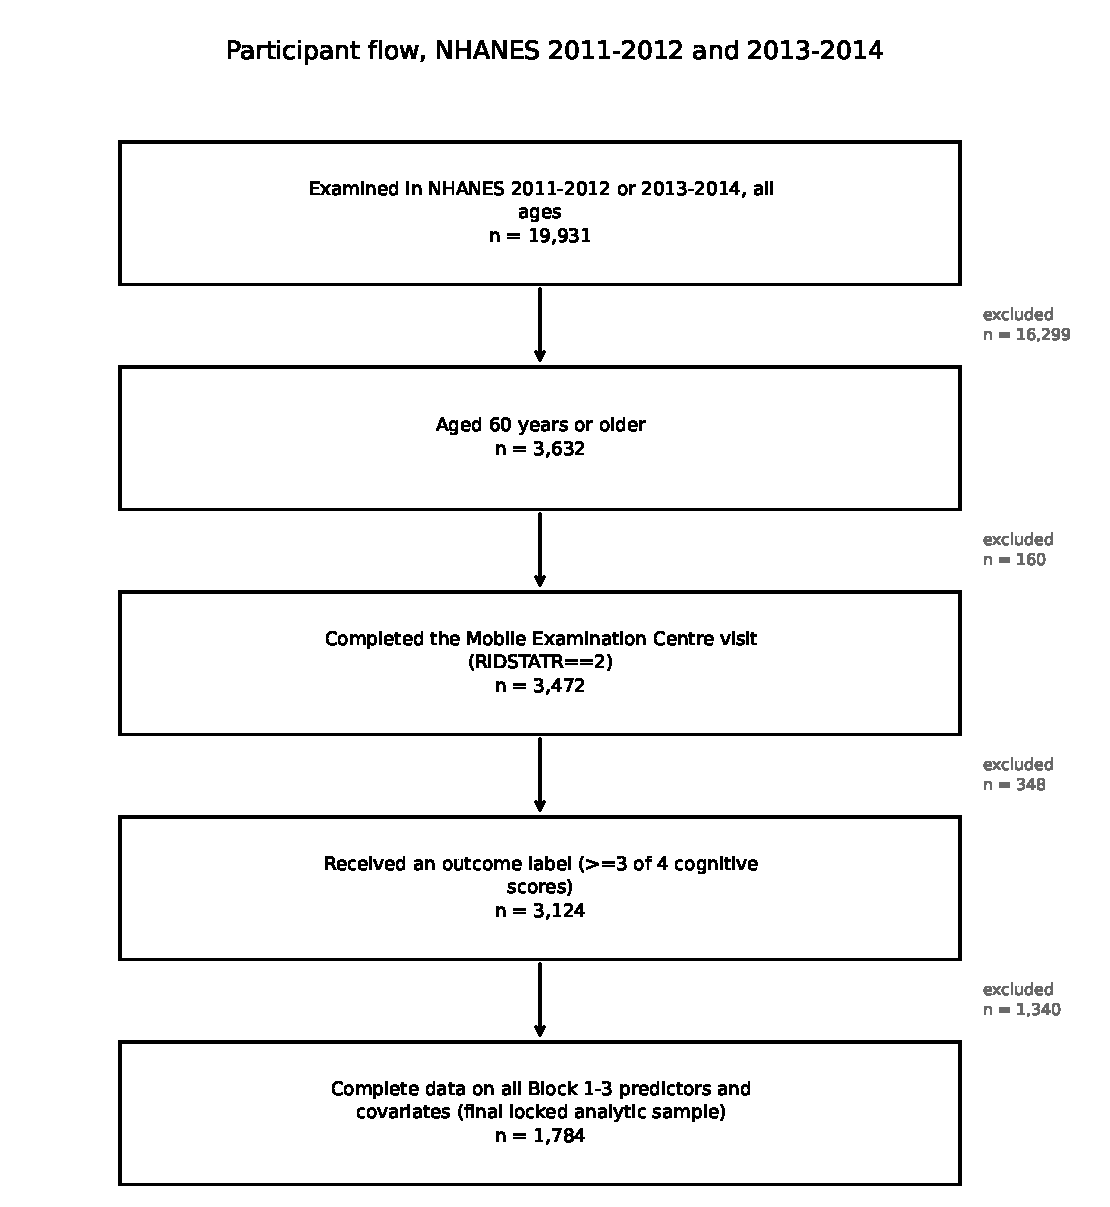
\includegraphics[width=0.85\textwidth]{figures/fig6_participant_flow.pdf}
\caption{Participant flow from NHANES 2011-2012 and 2013-2014 examined participants to the final locked analytic sample. Reasons for exclusion are given at each stage; the final step's exclusions (missing predictor data) are not mutually exclusive across blocks.}
\label{fig:flow}
\end{figure}

\begin{figure}[htbp]
\centering
\DIFdelbeginFL %DIFDELCMD < 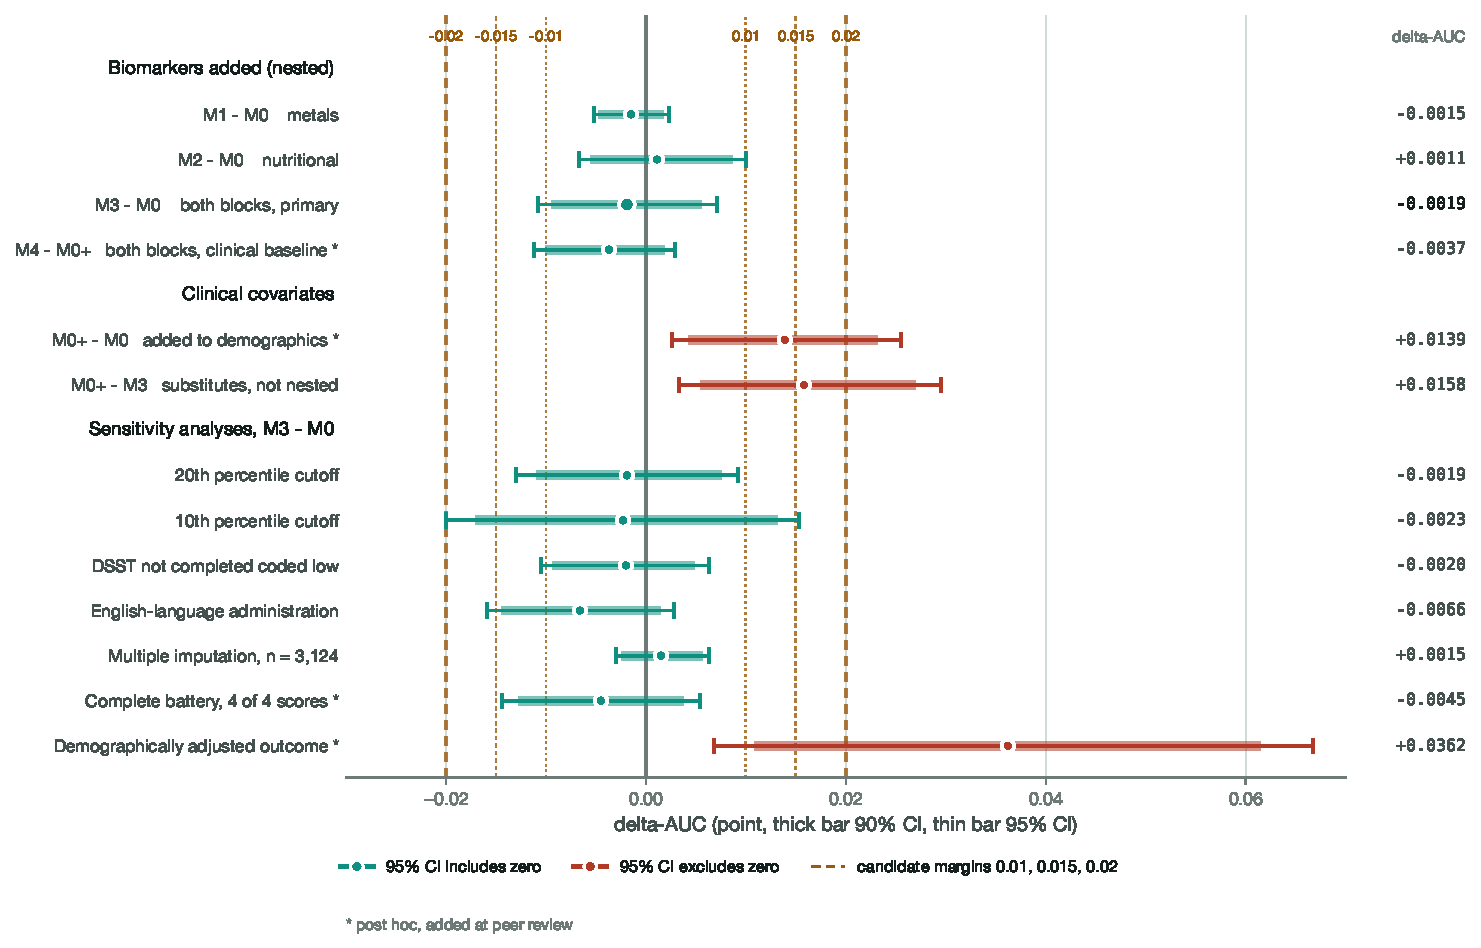
\includegraphics[width=0.95\textwidth]{figures/fig1_delta_auc_forest.pdf}
%DIFDELCMD < %%%
\DIFdelendFL \DIFaddbeginFL 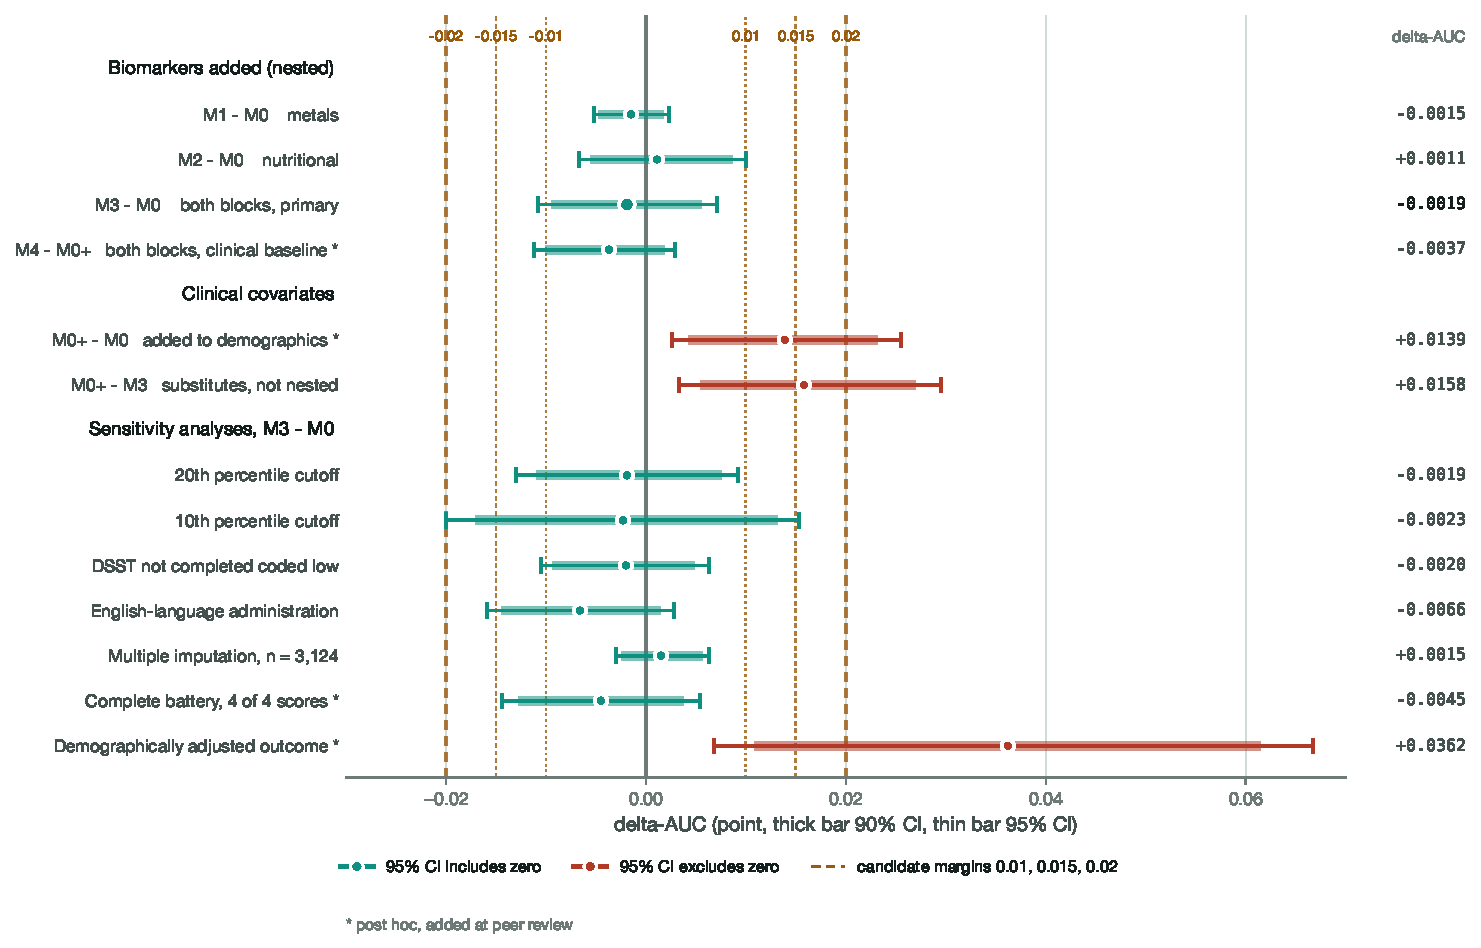
\includegraphics[width=0.98\textwidth]{figures/fig1_delta_auc_forest.pdf}
\DIFaddendFL \caption{Forest plot of \deltaauc\ contrasts \DIFaddbeginFL \DIFaddFL{under L2-penalized logistic regression, }\DIFaddendFL with \DIFdelbeginFL \DIFdelFL{bootstrap }\DIFdelendFL \DIFaddbeginFL \DIFaddFL{paired-bootstrap }\DIFaddendFL 95\% \DIFaddbeginFL \DIFaddFL{(thin bars) and 90\% (thick bars) }\DIFaddendFL confidence intervals\DIFaddbeginFL \DIFaddFL{. Top}\DIFaddendFL : \DIFdelbeginFL \DIFdelFL{the four primary }\DIFdelendFL \DIFaddbeginFL \DIFaddFL{biomarkers added to }\DIFaddendFL nested \DIFdelbeginFL \DIFdelFL{contrasts (M1$-$M0}\DIFdelendFL \DIFaddbeginFL \DIFaddFL{baselines}\DIFaddendFL , \DIFdelbeginFL \DIFdelFL{M2}\DIFdelendFL \DIFaddbeginFL \DIFaddFL{including M4 }\DIFaddendFL $-$ M0\DIFaddbeginFL \DIFaddFL{+. Middle: the clinical covariates added to demographics}\DIFaddendFL , \DIFdelbeginFL \DIFdelFL{M3$-$}\DIFdelendFL \DIFaddbeginFL \DIFaddFL{and the non-nested }\DIFaddendFL M0\DIFdelbeginFL \DIFdelFL{, }\DIFdelendFL \DIFaddbeginFL \DIFaddFL{+ against }\DIFaddendFL M3 \DIFaddbeginFL \DIFaddFL{contrast. Bottom: \deltaauc(M3 }\DIFaddendFL $-$ M0\DIFdelbeginFL \DIFdelFL{+}\DIFdelendFL ) \DIFdelbeginFL \DIFdelFL{and the six pre-specified }\DIFdelendFL \DIFaddbeginFL \DIFaddFL{under each }\DIFaddendFL sensitivity \DIFdelbeginFL \DIFdelFL{analyses for M3$-$M0}\DIFdelendFL \DIFaddbeginFL \DIFaddFL{analysis}\DIFaddendFL . \DIFaddbeginFL \DIFaddFL{Rows marked with an asterisk were added at peer review (post hoc). }\DIFaddendFL Red markers indicate \DIFaddbeginFL \DIFaddFL{95\% }\DIFaddendFL intervals excluding zero. \DIFdelbeginFL \DIFdelFL{The shaded band marks the pre-specified }\DIFdelendFL \DIFaddbeginFL \DIFaddFL{Dotted and dashed lines mark candidate margins of 0.01, 0.015 and }\DIFaddendFL 0.02 \DIFdelbeginFL \DIFdelFL{meaningful-difference threshold}\DIFdelendFL \DIFaddbeginFL \DIFaddFL{on both sides of zero; no margin is privileged}\DIFaddendFL .}
\label{fig:forest}
\end{figure}

\begin{figure}[htbp]
\centering
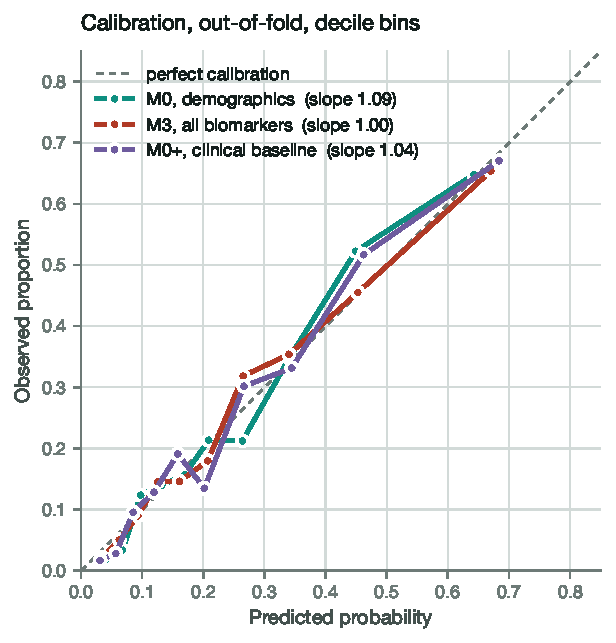
\includegraphics[width=0.7\textwidth]{figures/fig2_calibration.pdf}
\caption{Calibration, out-of-fold, by decile of predicted probability, for M0 (demographics), M3 (all biomarkers) and M0+ (\DIFdelbeginFL \DIFdelFL{clinical }\DIFdelendFL \DIFaddbeginFL \DIFaddFL{demographic-plus-clinical-history }\DIFaddendFL baseline). Calibration slope for each model is given in the legend; the dashed line is perfect calibration.}
\label{fig:calibration}
\end{figure}

\begin{figure}[htbp]
\centering
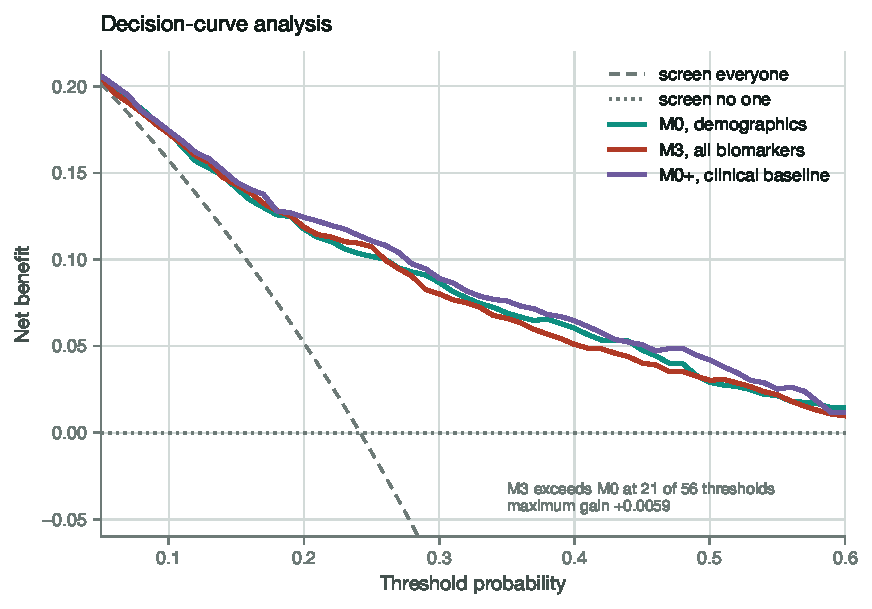
\includegraphics[width=0.85\textwidth]{figures/fig3_decision_curve.pdf}
\caption{Decision-curve analysis: net benefit against threshold probability for M0, M3 and M0+, against the treat-all and treat-none reference strategies.}
\label{fig:dca}
\end{figure}

\begin{figure}[htbp]
\centering
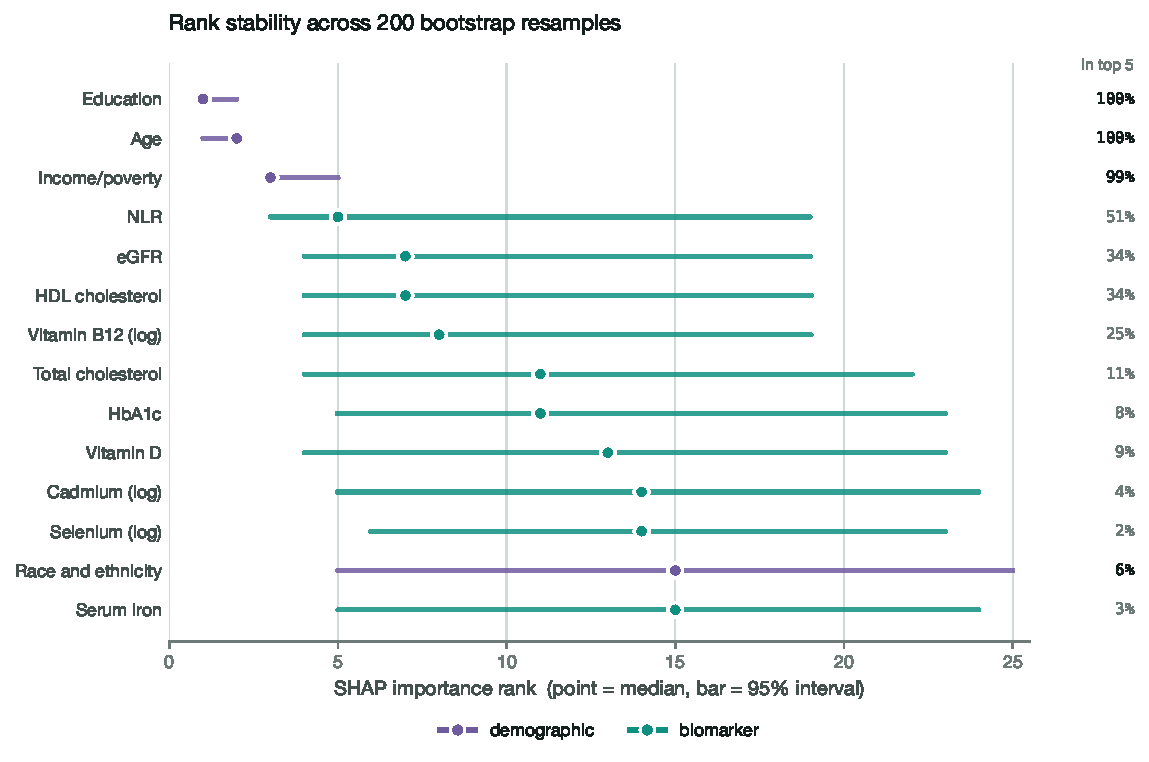
\includegraphics[width=0.9\textwidth]{figures/fig4_shap_rank_stability.pdf}
\caption{SHAP feature-importance rank stability across 200 bootstrap resamples of the gradient-boosted M3 model. Points are median rank, bars are the 95\% interval; the right-hand column gives the percentage of resamples in which each feature appeared in the top 5. \DIFdelbeginFL \DIFdelFL{Demographic predictors (purple) }\DIFdelendFL \DIFaddbeginFL \DIFaddFL{Education, age and the income-to-poverty ratio }\DIFaddendFL are essentially deterministic in rank; \DIFaddbeginFL \DIFaddFL{the }\DIFaddendFL biomarkers (teal)\DIFaddbeginFL \DIFaddFL{, and race and Hispanic origin and sex, }\DIFaddendFL are not.}
\label{fig:shap}
\end{figure}

\begin{figure}[htbp]
\centering
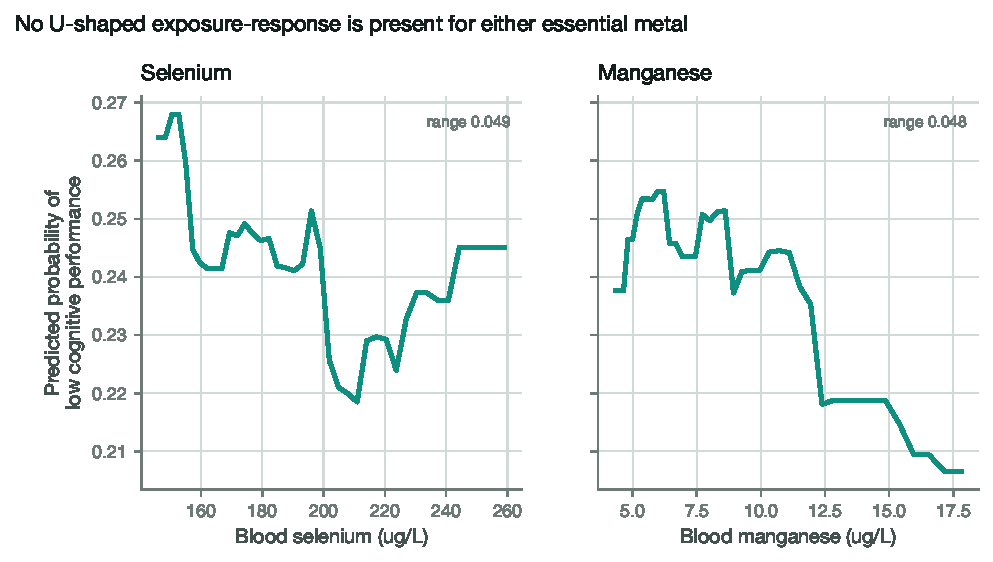
\includegraphics[width=0.9\textwidth]{figures/fig5_partial_dependence.pdf}
\caption{Partial dependence of predicted probability of low cognitive performance on blood selenium and blood manganese concentration (gradient-boosted M3 model), the two exposures for which a non-monotonic (U-shaped) exposure-response was anticipated in advance. Neither shows one; the predicted probability varies by approximately 0.05 across each exposure's observed range.}
\label{fig:pdp}
\end{figure}

\clearpage

% ============================================================
%DIF <  TABLE 1
%DIF >  TABLES
% ============================================================
\nolinenumbers
\begin{singlespace}
\footnotesize

\DIFdelbegin %DIFDELCMD < \begin{longtable}{p{6.6cm}R{2.6cm}R{2.6cm}R{2.6cm}}
%DIFDELCMD < \caption{Participant characteristics, analytic sample ($n=1{,}784$), overall and by outcome status.}
%DIFDELCMD < \label{tab:t1a}\\
%DIFDELCMD < \toprule
%DIFDELCMD < Characteristic & Overall & Low cognitive performance & Not low cognitive performance \\
%DIFDELCMD < \midrule
%DIFDELCMD < \endfirsthead
%DIFDELCMD < \multicolumn{4}{l}{\textit{Table \ref{tab:t1a} continued}}\\
%DIFDELCMD < \toprule
%DIFDELCMD < Characteristic & Overall & Low cognitive performance & Not low cognitive performance \\
%DIFDELCMD < \midrule
%DIFDELCMD < \endhead
%DIFDELCMD < \bottomrule
%DIFDELCMD < \endfoot
%DIFDELCMD < \bottomrule
%DIFDELCMD < \endlastfoot
%DIFDELCMD < $n$ & 1784 & 431 & 1353 \\
%DIFDELCMD < Age, years, mean (SD) & 69.37 (6.74) & 72.07 (6.94) & 68.52 (6.44) \\
%DIFDELCMD < Income-to-poverty ratio, mean (SD) & 2.60 (1.60) & 1.91 (1.38) & 2.82 (1.61) \\
%DIFDELCMD < Blood lead, $\mu$g/dL, median [IQR] & 1.47 [1.01, 2.19] & 1.57 [1.03, 2.41] & 1.44 [1.01, 2.12] \\
%DIFDELCMD < Blood cadmium, $\mu$g/L, median [IQR] & 0.38 [0.25, 0.61] & 0.42 [0.27, 0.69] & 0.37 [0.25, 0.58] \\
%DIFDELCMD < Blood total mercury, $\mu$g/L, median [IQR] & 0.93 [0.49, 1.94] & 0.75 [0.40, 1.56] & 0.99 [0.53, 2.01] \\
%DIFDELCMD < Blood selenium, $\mu$g/L, median [IQR] & 193.09 [177.40, 208.38] & 188.35 [173.17, 204.15] & 194.23 [179.15, 209.06] \\
%DIFDELCMD < Blood manganese, $\mu$g/L, median [IQR] & 8.71 [6.90, 11.09] & 8.35 [6.50, 10.69] & 8.80 [7.02, 11.19] \\
%DIFDELCMD < Serum vitamin B12, pmol/L, median [IQR] & 410.30 [289.30, 601.45] & 421.40 [284.50, 621.80] & 408.10 [290.00, 599.30] \\
%DIFDELCMD < Serum methylmalonic acid, $\mu$mol/L, median [IQR] & 163.00 [125.75, 227.00] & 181.00 [131.00, 256.00] & 160.00 [124.00, 214.00] \\
%DIFDELCMD < Serum total folate, nmol/L, median [IQR] & 20.80 [13.60, 31.42] & 20.00 [13.05, 32.05] & 20.90 [13.70, 31.30] \\
%DIFDELCMD < RBC folate, nmol/L, median [IQR] & 543.00 [398.00, 737.00] & 530.00 [391.00, 748.50] & 547.00 [401.00, 733.00] \\
%DIFDELCMD < 25-hydroxyvitamin D, nmol/L, mean (SD) & 76.31 (30.44) & 72.68 (30.36) & 77.46 (30.39) \\
%DIFDELCMD < HbA1c, \%, median [IQR] & 5.80 [5.50, 6.30] & 5.90 [5.50, 6.50] & 5.80 [5.50, 6.20] \\
%DIFDELCMD < HDL cholesterol, mg/dL, median [IQR] & 52.00 [43.00, 63.00] & 49.00 [40.00, 60.00] & 52.00 [44.00, 63.00] \\
%DIFDELCMD < Total cholesterol, mg/dL, mean (SD) & 192.85 (43.15) & 185.58 (41.41) & 195.16 (43.45) \\
%DIFDELCMD < Triglycerides, mg/dL, median [IQR] & 126.00 [86.00, 187.25] & 128.00 [91.00, 182.00] & 126.00 [85.00, 189.00] \\
%DIFDELCMD < Serum albumin, g/dL, mean (SD) & 4.20 (0.31) & 4.15 (0.34) & 4.21 (0.29) \\
%DIFDELCMD < Serum iron, $\mu$g/dL, median [IQR] & 80.00 [61.00, 103.00] & 76.00 [57.00, 96.00] & 82.00 [63.00, 104.00] \\
%DIFDELCMD < eGFR, mL/min/1.73\,m\textsuperscript{2}, mean (SD) & 75.64 (19.85) & 69.95 (22.19) & 77.45 (18.69) \\
%DIFDELCMD < Neutrophil-to-lymphocyte ratio, median [IQR] & 2.11 [1.55, 2.92] & 2.35 [1.67, 3.21] & 2.05 [1.53, 2.83] \\
%DIFDELCMD < Platelet-to-lymphocyte ratio, median [IQR] & 119.80 [94.11, 152.96] & 119.05 [89.76, 153.87] & 120.00 [95.26, 152.50] \\
%DIFDELCMD < Systemic immune-inflammation index, median [IQR] & 458.83 [319.14, 664.17] & 480.65 [322.90, 714.20] & 452.00 [315.00, 646.00] \\
%DIFDELCMD < Body mass index, kg/m\textsuperscript{2}, median [IQR] & 28.10 [24.77, 32.40] & 27.60 [24.30, 31.90] & 28.20 [24.90, 32.50] \\
%DIFDELCMD < Alcoholic drinks per day, median [IQR] & 0.00 [0.00, 1.25] & 0.00 [0.00, 1.00] & 1.00 [0.00, 2.00] \\
%DIFDELCMD < PHQ-9 depression score, median [IQR] & 1.00 [0.00, 4.00] & 2.00 [0.00, 6.50] & 1.00 [0.00, 4.00] \\
%DIFDELCMD < Sex = Male & 880 (49.3\%) & 238 (55.2\%) & 642 (47.5\%) \\
%DIFDELCMD < Sex = Female & 904 (50.7\%) & 193 (44.8\%) & 711 (52.5\%) \\
%DIFDELCMD < Race/ethnicity = Mexican American & 140 (7.8\%) & 46 (10.7\%) & 94 (6.9\%) \\
%DIFDELCMD < Race/ethnicity = Other Hispanic & 182 (10.2\%) & 68 (15.8\%) & 114 (8.4\%) \\
%DIFDELCMD < Race/ethnicity = Non-Hispanic White & 863 (48.4\%) & 165 (38.3\%) & 698 (51.6\%) \\
%DIFDELCMD < Race/ethnicity = Non-Hispanic Black & 425 (23.8\%) & 120 (27.8\%) & 305 (22.5\%) \\
%DIFDELCMD < Race/ethnicity = Non-Hispanic Asian & 144 (8.1\%) & 26 (6.0\%) & 118 (8.7\%) \\
%DIFDELCMD < Race/ethnicity = Other/multiracial & 30 (1.7\%) & 6 (1.4\%) & 24 (1.8\%) \\
%DIFDELCMD < Education = Less than 9th grade & 224 (12.6\%) & 137 (31.8\%) & 87 (6.4\%) \\
%DIFDELCMD < Education = 9-11th grade & 219 (12.3\%) & 79 (18.3\%) & 140 (10.3\%) \\
%DIFDELCMD < Education = High school grad/GED & 417 (23.4\%) & 103 (23.9\%) & 314 (23.2\%) \\
%DIFDELCMD < Education = Some college/AA degree & 511 (28.6\%) & 71 (16.5\%) & 440 (32.5\%) \\
%DIFDELCMD < Education = College graduate or above & 413 (23.2\%) & 41 (9.5\%) & 372 (27.5\%) \\
%DIFDELCMD < Smoking status = Never & 895 (50.2\%) & 210 (48.7\%) & 685 (50.6\%) \\
%DIFDELCMD < Smoking status = Former & 671 (37.6\%) & 159 (36.9\%) & 512 (37.8\%) \\
%DIFDELCMD < Smoking status = Current & 218 (12.2\%) & 62 (14.4\%) & 156 (11.5\%) \\
%DIFDELCMD < Ever told had a stroke & 125 (7.0\%) & 49 (11.4\%) & 76 (5.6\%) \\
%DIFDELCMD < Ever told had diabetes & 490 (27.5\%) & 154 (35.7\%) & 336 (24.8\%) \\
%DIFDELCMD < Ever told had high blood pressure & 1111 (62.3\%) & 302 (70.1\%) & 809 (59.8\%) \\
%DIFDELCMD < Ever told had high cholesterol & 997 (55.9\%) & 234 (54.3\%) & 763 (56.4\%) \\
%DIFDELCMD < \end{longtable}
%DIFDELCMD < %%%
\DIFdelend \DIFaddbegin \begin{longtable}{L{4.6cm}R{3.35cm}R{3.35cm}R{3.35cm}}
\caption{Participant characteristics, analytic sample ($n=1{,}784$), overall and by outcome status. Cognitive scores are raw scores; the composite is the mean of the available within-sample z-scores.}
\label{tab:t1a}\\
\toprule
Characteristic & Overall & Low cognitive performance & Not low cognitive performance \\
\midrule
\endfirsthead
\multicolumn{4}{l}{\textit{Table \ref{tab:t1a} continued}}\\
\toprule
Characteristic & Overall & Low cognitive performance & Not low cognitive performance \\
\midrule
\endhead
\bottomrule
\endfoot
\bottomrule
\endlastfoot
$n$ & 1784 & 431 & 1353 \\
\multicolumn{4}{l}{\textit{Cognitive measures}}\\
CERAD immediate recall (sum of 3 trials, 0 to 30), mean (SD) & 18.52 (4.87) & 12.88 (3.82) & 20.32 (3.63) \\
\quad score missing, $n$ (\%) & 3 (0.2\%) & 0 (0.0\%) & 3 (0.2\%) \\
CERAD delayed recall (0 to 10), mean (SD) & 5.77 (2.40) & 3.07 (1.88) & 6.62 (1.85) \\
\quad score missing, $n$ (\%) & 3 (0.2\%) & 2 (0.5\%) & 1 (0.1\%) \\
Animal fluency (animals named in 60 s), mean (SD) & 16.54 (5.52) & 11.55 (3.51) & 18.10 (5.10) \\
\quad score missing, $n$ (\%) & 20 (1.1\%) & 11 (2.6\%) & 9 (0.7\%) \\
Digit Symbol Substitution Test (correct symbols), mean (SD) & 46.31 (17.24) & 28.68 (11.27) & 51.42 (15.17) \\
\quad score missing, $n$ (\%) & 64 (3.6\%) & 45 (10.4\%) & 19 (1.4\%) \\
Composite z-score, mean (SD) & 0.01 (0.79) & $-$1.04 (0.41) & 0.34 (0.55) \\
Composite z-score, median [IQR] & 0.04 [$-$0.52, 0.56] & $-$0.93 [$-$1.26, $-$0.71] & 0.29 [$-$0.09, 0.71] \\
Composite z-score, range & $-$2.43 to 2.45 & $-$2.43 to $-$0.55 & $-$0.54 to 2.45 \\
Language of administration = English & 1575 (88.3\%) & 345 (80.0\%) & 1230 (90.9\%) \\
Language of administration = Spanish & 174 (9.8\%) & 79 (18.3\%) & 95 (7.0\%) \\
Language of administration = Asian language & 35 (2.0\%) & 7 (1.6\%) & 28 (2.1\%) \\
Component scores = 4 & 1694 (95.0\%) & 373 (86.5\%) & 1321 (97.6\%) \\
Component scores = 3 & 90 (5.0\%) & 58 (13.5\%) & 32 (2.4\%) \\
Outcome cutoff (lowest quartile of the 3,124 labelled participants) & \multicolumn{3}{r}{composite $z \le -0.543$} \\
\multicolumn{4}{l}{\textit{Demographic, laboratory and clinical characteristics}}\\
Age, years, mean (SD) & 69.37 (6.74) & 72.07 (6.94) & 68.52 (6.44) \\
Income-to-poverty ratio, mean (SD) & 2.60 (1.60) & 1.91 (1.38) & 2.82 (1.61) \\
Blood lead, $\mu$g/dL, median [IQR] & 1.47 [1.01, 2.19] & 1.57 [1.03, 2.41] & 1.44 [1.01, 2.12] \\
Blood cadmium, $\mu$g/L, median [IQR] & 0.38 [0.25, 0.61] & 0.42 [0.27, 0.69] & 0.37 [0.25, 0.58] \\
Blood total mercury, $\mu$g/L, median [IQR] & 0.93 [0.49, 1.94] & 0.75 [0.40, 1.56] & 0.99 [0.53, 2.01] \\
Blood selenium, $\mu$g/L, median [IQR] & 193.09 [177.40, 208.38] & 188.35 [173.17, 204.15] & 194.23 [179.15, 209.06] \\
Blood manganese, $\mu$g/L, median [IQR] & 8.71 [6.90, 11.09] & 8.35 [6.50, 10.69] & 8.80 [7.02, 11.19] \\
Serum vitamin B12, pmol/L, median [IQR] & 410.30 [289.30, 601.45] & 421.40 [284.50, 621.80] & 408.10 [290.00, 599.30] \\
Serum methylmalonic acid, $\mu$mol/L, median [IQR] & 163.00 [125.75, 227.00] & 181.00 [131.00, 256.00] & 160.00 [124.00, 214.00] \\
Serum total folate, nmol/L, median [IQR] & 20.80 [13.60, 31.42] & 20.00 [13.05, 32.05] & 20.90 [13.70, 31.30] \\
RBC folate, nmol/L, median [IQR] & 543.00 [398.00, 737.00] & 530.00 [391.00, 748.50] & 547.00 [401.00, 733.00] \\
25-hydroxyvitamin D, nmol/L, mean (SD) & 76.31 (30.44) & 72.68 (30.36) & 77.46 (30.39) \\
HbA1c, \%, median [IQR] & 5.80 [5.50, 6.30] & 5.90 [5.50, 6.50] & 5.80 [5.50, 6.20] \\
HDL cholesterol, mg/dL, median [IQR] & 52.00 [43.00, 63.00] & 49.00 [40.00, 60.00] & 52.00 [44.00, 63.00] \\
Total cholesterol, mg/dL, mean (SD) & 192.85 (43.15) & 185.58 (41.41) & 195.16 (43.45) \\
Triglycerides, mg/dL, median [IQR] & 126.00 [86.00, 187.25] & 128.00 [91.00, 182.00] & 126.00 [85.00, 189.00] \\
Serum albumin, g/dL, mean (SD) & 4.20 (0.31) & 4.15 (0.34) & 4.21 (0.29) \\
Serum iron, $\mu$g/dL, median [IQR] & 80.00 [61.00, 103.00] & 76.00 [57.00, 96.00] & 82.00 [63.00, 104.00] \\
eGFR, mL/min/1.73\,m\textsuperscript{2}, mean (SD) & 75.64 (19.85) & 69.95 (22.19) & 77.45 (18.69) \\
Neutrophil-to-lymphocyte ratio, median [IQR] & 2.11 [1.55, 2.92] & 2.35 [1.67, 3.21] & 2.05 [1.53, 2.83] \\
Platelet-to-lymphocyte ratio, median [IQR] & 119.80 [94.11, 152.96] & 119.05 [89.76, 153.87] & 120.00 [95.26, 152.50] \\
Systemic immune-inflammation index, median [IQR] & 458.83 [319.14, 664.17] & 480.65 [322.90, 714.20] & 452.00 [315.00, 646.00] \\
Body mass index, kg/m\textsuperscript{2}, median [IQR] & 28.10 [24.77, 32.40] & 27.60 [24.30, 31.90] & 28.20 [24.90, 32.50] \\
Alcoholic drinks per day, median [IQR] & 0.00 [0.00, 1.25] & 0.00 [0.00, 1.00] & 1.00 [0.00, 2.00] \\
PHQ-9 depression score, median [IQR] & 1.00 [0.00, 4.00] & 2.00 [0.00, 6.50] & 1.00 [0.00, 4.00] \\
Sex = Male & 880 (49.3\%) & 238 (55.2\%) & 642 (47.5\%) \\
Sex = Female & 904 (50.7\%) & 193 (44.8\%) & 711 (52.5\%) \\
Race/ethnicity = Mexican American & 140 (7.8\%) & 46 (10.7\%) & 94 (6.9\%) \\
Race/ethnicity = Other Hispanic & 182 (10.2\%) & 68 (15.8\%) & 114 (8.4\%) \\
Race/ethnicity = Non-Hispanic White & 863 (48.4\%) & 165 (38.3\%) & 698 (51.6\%) \\
Race/ethnicity = Non-Hispanic Black & 425 (23.8\%) & 120 (27.8\%) & 305 (22.5\%) \\
Race/ethnicity = Non-Hispanic Asian & 144 (8.1\%) & 26 (6.0\%) & 118 (8.7\%) \\
Race/ethnicity = Other/multiracial & 30 (1.7\%) & 6 (1.4\%) & 24 (1.8\%) \\
Education = Less than 9th grade & 224 (12.6\%) & 137 (31.8\%) & 87 (6.4\%) \\
Education = 9 to 11th grade & 219 (12.3\%) & 79 (18.3\%) & 140 (10.3\%) \\
Education = High school grad/GED & 417 (23.4\%) & 103 (23.9\%) & 314 (23.2\%) \\
Education = Some college/AA degree & 511 (28.6\%) & 71 (16.5\%) & 440 (32.5\%) \\
Education = College graduate or above & 413 (23.2\%) & 41 (9.5\%) & 372 (27.5\%) \\
Smoking status = Never & 895 (50.2\%) & 210 (48.7\%) & 685 (50.6\%) \\
Smoking status = Former & 671 (37.6\%) & 159 (36.9\%) & 512 (37.8\%) \\
Smoking status = Current & 218 (12.2\%) & 62 (14.4\%) & 156 (11.5\%) \\
Ever told had a stroke & 125 (7.0\%) & 49 (11.4\%) & 76 (5.6\%) \\
Ever told had diabetes & 490 (27.5\%) & 154 (35.7\%) & 336 (24.8\%) \\
Ever told had high blood pressure & 1111 (62.3\%) & 302 (70.1\%) & 809 (59.8\%) \\
Ever told had high cholesterol & 997 (55.9\%) & 234 (54.3\%) & 763 (56.4\%) \\
\end{longtable}
\DIFaddend 

\bigskip

\begin{longtable}{p{6.0cm}R{3.5cm}R{3.5cm}}
\caption{Included versus excluded participants, among the 3,124 outcome-eligible participants.}
\label{tab:t1b}\\
\toprule
Characteristic & Included ($n=1{,}784$) & Excluded ($n=1{,}340$) \\
\midrule
\endfirsthead
\toprule
Characteristic & Included ($n=1{,}784$) & Excluded ($n=1{,}340$) \\
\midrule
\endhead
\bottomrule
\endlastfoot
Age, years, mean (SD) & 69.37 (6.74) & 70.10 (6.94) \\
Income-to-poverty ratio, mean (SD) & 2.60 (1.60) & 2.50 (1.59) \\
PHQ-9 depression score, median [IQR] & 1.00 [0.00, 4.00] & 2.00 [0.00, 5.00] \\
Female, \% & 50.7\% & 52.6\% \\
Low cognitive performance, \% & 24.2\% & 26.1\% \\
Diabetes, \% & 27.5\% & 30.0\% \\
\end{longtable}

\DIFaddbegin \bigskip

{\setlength{\tabcolsep}{3pt}
\begin{longtable}{L{3.0cm}L{1.9cm}R{1.3cm}R{2.9cm}R{2.9cm}R{0.85cm}R{0.85cm}R{0.85cm}}
\caption{Incremental discrimination under L2-penalized logistic regression, with margin analysis. \deltaauc\ with paired-bootstrap 95\% and 90\% intervals (2,000 resamples). The last three columns state whether the 90\% interval lies wholly within $\pm\delta$ (equivalence by two one-sided tests at $\alpha = 0.05$) for $\delta$ = 0.01, 0.015 and 0.02. The margin analysis, M4 and the M0+ $-$ M0 contrast were added at peer review (post hoc); the M4 $-$ M0+ lower 90\% bound is $-0.00997$, shown rounded; the 0.02 value was declared in advance without external justification and no margin is privileged. Sensitivity analyses are in Additional file 4 (Table S8) and every pairwise contrast under every algorithm in Table S6.}
\label{tab:t3}\\
\toprule
& & & & & \multicolumn{3}{c}{Within $\pm\delta$} \\
\cmidrule(l){6-8}
Contrast & & \deltaauc & 95\% CI & 90\% CI & 0.01 & 0.015 & 0.02 \\
\midrule
\endfirsthead
\toprule
& & & & & \multicolumn{3}{c}{Within $\pm\delta$} \\
\cmidrule(l){6-8}
Contrast & & \deltaauc & 95\% CI & 90\% CI & 0.01 & 0.015 & 0.02 \\
\midrule
\endhead
\bottomrule
\endlastfoot
Metals added to demographics & M1 $-$ M0 & $-0.0015$ & [$-0.0052$, 0.0023] & [$-0.0047$, 0.0018] & yes & yes & yes \\
Nutritional and metabolic biomarkers added to demographics & M2 $-$ M0 & 0.0011 & [$-0.0067$, 0.0100] & [$-0.0055$, 0.0087] & yes & yes & yes \\
Both biomarker blocks added to demographics (primary) & M3 $-$ M0 & $-0.0019$ & [$-0.0108$, 0.0071] & [$-0.0094$, 0.0056] & yes & yes & yes \\
Clinical covariates added to demographics (post hoc) & M0+ $-$ M0 & 0.0139 & [0.0026, 0.0255] & [0.0043, 0.0232] & no & no & no \\
Both biomarker blocks added to the clinical baseline (post hoc) & M4 $-$ M0+ & $-0.0037$ & [$-0.0112$, 0.0029] & [$-0.0100$, 0.0019] & yes & yes & yes \\
Clinical baseline against biomarker model (substitutes) & M0+ $-$ M3 & 0.0158 & [0.0033, 0.0295] & [0.0055, 0.0270] & no & no & no \\
\end{longtable}
}

\DIFaddend \end{singlespace}
\linenumbers

\clearpage

\doublespacing

% ============================================================
% DECLARATIONS
% ============================================================
\section*{Declarations}

\subsection*{Ethics approval and consent to participate}

NHANES protocol and procedures were approved by the National Center for Health Statistics (NCHS) Ethics Review Board (formerly the NCHS Research Ethics Review Board), and written informed consent was obtained from all participants by NCHS prior to data collection. This study is a secondary analysis of de-identified, publicly available data and involved no additional contact with participants. Both authors confirmed that their institutions (Davidson College and the University of North Carolina at Chapel Hill) impose no additional IRB requirement for this secondary analysis.

\subsection*{Consent for publication}

Not applicable. No individual person's data, images, or identifiable information are presented; all results are reported at the level of aggregate statistics on a de-identified public dataset.

\subsection*{Availability of data and materials}

NHANES data are publicly available from the CDC at wwwn.cdc.gov and are not redistributed here; the download script rebuilds the raw dataset from the original CDC URLs. The analysis code\DIFaddbegin \DIFadd{, including the scripts for every analysis added at peer review, }\DIFaddend is available at \url{https://github.com/NeilP211/nhanes-ieee}, under version control, with every random seed fixed and every package version pinned.

\subsection*{Competing interests}

The authors declare that they have no competing interests.

\subsection*{Funding}

This research received no specific grant from any funding agency in the public, commercial, or not-for-profit sectors.

\subsection*{Authors' contributions}

S.K.\ and N.P.\ conceived the study and jointly decided the analytic sample definition, the nested model specification, and the pre-registration. S.K.\ acquired the raw data. N.P.\ curated the data and developed and ran the primary modelling pipeline: cohort construction, outcome construction, the nested \DIFdelbegin \DIFdel{M0-M3/}\DIFdelend M0 \DIFaddbegin \DIFadd{to M3 and M0}\DIFaddend + models across three algorithms, cross-validated evaluation, interpretation (SHAP, partial dependence), and the six sensitivity analyses. S.K.\ conducted the literature review and citation verification, and conducted the participant flow-diagram, Table~\ref{tab:t1a}, and full model coefficient analyses. N.P.\ wrote the original draft of the Methods and Results; S.K.\ wrote the original draft of the Abstract, Background, and Discussion. \DIFdelbegin \DIFdel{Both authors }\DIFdelend \DIFaddbegin \DIFadd{N.P.\ conducted the analyses added at peer review. Both authors revised the manuscript in response to peer review, }\DIFaddend reviewed and edited the complete manuscript\DIFaddbegin \DIFadd{, }\DIFaddend and approved the final version. S.K.\ and N.P.\ contributed equally to this work and share first authorship.

\subsection*{Acknowledgements}

Not applicable.

% ============================================================
% REFERENCES
% ============================================================
\clearpage
\begin{singlespace}
\section*{References}

\begin{enumerate}
\item Wang N, Guo L, Shi M, Wang L, Zhou Y, Liu H, et al. Association of single and combined effects of blood heavy metals with cognitive function in older adults of the United States: a cross-sectional study. Research Square [Preprint]. 2024. \DIFdelbegin \DIFdel{Not confirmed as peer-reviewed at time of writing, cite as a preprint. }\DIFdelend Available from: \url{https://www.researchsquare.com/article/rs-4786268/v1}

\item Lu K, Liu T, Wu X, Zhong J, Ou Z, Wu W. Association between serum iron, blood lead, cadmium, mercury, selenium, manganese and low cognitive performance in old adults from National Health and Nutrition Examination Survey (NHANES): a cross-sectional study. Br J Nutr. 2023;130(10):1743-1753. \url{https://doi.org/10.1017/S0007114523000740}

\item Tang C, Shen M, Hong H. Uncovering the relationship between trace element exposure, cognitive function, and dietary inflammation index in elderly Americans from the National Health and Nutrition Examination Survey 2011-2014. BMC Public Health. 2024;24:2516. \url{https://doi.org/10.1186/s12889-024-20060-4}

\item Fu Z, Xu X, Cao L, Xiang Q, Gao Q, Duan H, et al. Single and joint exposure of Pb, Cd, Hg, Se, Cu, and Zn were associated with cognitive function of older adults. Sci Rep. 2024;14:28567. \url{https://doi.org/10.1038/s41598-024-79720-5}

\item Song S, Liu N, Wang G, Wang Y, Zhang X, Zhao X, et al. Sex specificity in the mixed effects of blood heavy metals and cognitive function on elderly: evidence from NHANES. Nutrients. 2023;15(13):2874. \url{https://doi.org/10.3390/nu15132874}

\item Laouali N, Benmarhnia T, Lanphear BP, Weuve J, Mascari M, Boutron-Ruault MC, et al. Association between blood metals mixtures concentrations and cognitive performance, and effect modification by diet in older US adults. Environ Epidemiol. 2022;6(1):e192. \url{https://doi.org/10.1097/EE9.0000000000000192}

\item Huang G, Ren G. Interaction between omega-6 fatty acids intake and blood cadmium on the risk of low cognitive performance in older adults from National Health and Nutrition Examination Survey (NHANES) 2011-2014. BMC Geriatr. 2022. \url{https://doi.org/10.1186/s12877-022-02988-7}

\item Ren F, Zhao X, Yang Q, Liao H, Zhang Y, Liu X. A machine learning framework for predicting cognitive impairment in aging populations using urinary metal and demographic data. Front Genet. 2025;16:1631228. \url{https://doi.org/10.3389/fgene.2025.1631228}

\item Nabavi A, Safari F, Kashkooli M, Nabavizadeh SS, Molavi Vardanjani H. Early prediction of cognitive impairment in adults aged 20 years and older using machine learning and biomarkers of heavy metal exposure. Curr Res Toxicol. 2024;7:100198. \url{https://doi.org/10.1016/j.crtox.2024.100198}

\item \DIFaddbegin \DIFadd{Pepe MS, Janes H, Longton G, Leisenring W, Newcomb P. Limitations of the odds ratio in gauging the performance of a diagnostic, prognostic, or screening marker. Am J Epidemiol. 2004;159(9):882-890. }\url{https://doi.org/10.1093/aje/kwh101}

\item \DIFadd{Cook NR. Use and misuse of the receiver operating characteristic curve in risk prediction. Circulation. 2007;115(7):928-935. }\url{https://doi.org/10.1161/CIRCULATIONAHA.106.672402}

\item \DIFaddend Collins GS, Moons KGM, Dhiman P, Riley RD, Beam AL, Van Calster B, et al. TRIPOD+AI statement: updated guidance for reporting clinical prediction models that use regression or machine learning methods. BMJ. 2024;385:e078378. \url{https://doi.org/10.1136/bmj-2023-078378}
\DIFaddbegin 

\item \DIFadd{Walker E, Nowacki AS. Understanding equivalence and noninferiority testing. J Gen Intern Med. 2011;26(2):192-196. }\url{https://doi.org/10.1007/s11606-010-1513-8}

\item \DIFadd{Lakens D, Scheel AM, Isager PM. Equivalence testing for psychological research: a tutorial. Adv Methods Pract Psychol Sci. 2018;1(2):259-269. }\url{https://doi.org/10.1177/2515245918770963}

\item \DIFadd{Manly JJ, Jacobs DM, Touradji P, Small SA, Stern Y. Reading level attenuates differences in neuropsychological test performance between African American and White elders. J Int Neuropsychol Soc. 2002;8(3):341-348. }\url{https://doi.org/10.1017/S1355617702813157}
\DIFaddend 

\end{enumerate}
\end{singlespace}

\end{document}
